\documentclass[
    %Tamanho da fonte do documento
    12pt, 
    %Capítulos começam em página ímpar (insere uma página caso necessário)
    openright,
    %Impressão em frente e verso - oposto de oneside
    oneside, 
    %tamanho da página
    a4paper, 
    %Configurações opcionais
    %Altera para maiúscula as fontes dos capítulos
    chapter = title, 
    %Altera para maiúscula as fontes das seções
    section = title, 
    %Altera para maiúscula as fontes das subseções
    subsection = title, 
    %Altera para maiúscula as fontes das sub-subseções
    subsubsection = title,  
    %Idiomas para hifenização
    engish,
    brazil %Último idioma é a língua do documento
]{abntex2}


%Pacotes utilizados em citações
\usepackage[brazilian,hyperpageref]{backref}	 % Paginas com as citações na referência
\usepackage[alf]{abntex2cite}	                 % Citações padrão ABNT
\usepackage{titlesec}
%Inclusão de pacotes básicos
\usepackage{times}
\usepackage[T1]{fontenc}	% Seleção de códigos de fonte
\usepackage{lastpage}		% Usado pela Ficha catalográfica
\usepackage{indentfirst}	% Indenta o primeiro parágrafo de cada seção
\usepackage{color}			% Controle das cores
\usepackage{graphicx}		% Inclusão de gráficos
\usepackage{microtype} 		% para melhorias de justificação
\usepackage{enumitem}       %alíneas
\usepackage[utf8]{inputenc} %Codificação do documento UTF8 permite a utilização de acentos
\usepackage{float}
\usepackage{tocloft}        %usado para criar uma nota lista (lista de equações)
\usepackage{minted}
\usepackage{booktabs}
\usepackage{multirow}

%formatação dos capítulos, seções e subseções
\titleformat{\chapter}{\normalfont\large\bfseries}{\thechapter}{12pt}{\MakeUppercase}{\large}\titlespacing*{\chapter}{0pt}{10pt}{15pt}
\titleformat{\section}{\normalfont\large}{\thesection}{12pt}{\MakeUppercase}{}
\titleformat{\subsection}{\normalfont\large\bfseries}{\thesubsection}{12pt}{}
\titleformat{\subsubsection}{\normalfont\normalsize}{\thesubsubsection}{12pt}{}


% Configurações do pacote backref
% Usado sem a opção hyperpageref de backref
\renewcommand{\backrefpagesname}{Citado na(s) página(s):~} % Texto padrão antes do número das páginas
\renewcommand{\backref}{}
% Define os textos da citação
\renewcommand*{\backrefalt}[4]{
	\ifcase #1 % Caso adicione alguma bibliografia sem citação
		Nenhuma citação no texto.%
	\or
		Citado na página #2.%
	\else
		Citado #1 vezes nas páginas #2.%
	\fi}

%Informações do documento

\titulo{Ferramenta computacional para aproximação dinâmica da equação de chuva intensa por meio de redes neurais artificiais}
\autor{Erick Hardt \\ Fernando Longuini da Silva \\ João Pedro Lang Ramalho \\ Matheus Swerts Neder Miranda}
\local{Brasil}
\data{2018}
\orientador{Pedro Henrique Cerento de Lyra}
\coorientador{Carlos Alberto de Moya Figueira Netto}

\definecolor{blue}{RGB}{41,5,195} %Define a cor azul do texto

\preambulo{Trabalho de Graduação apresentado à Escola de Engenharia Mauá do Centro Universitário do Instituto Mauá de Tecnologia como requisito parcial para a obtenção de título de Engenheiro Civil. \newline Área de Concentração: Engenharia civil}

%Configurações de links do documento
\makeatletter %Permite a utilização do @ como macros
\hypersetup{
     	%pagebackref=true,
		pdftitle={\@title}, 
		pdfauthor={\@author},
    	pdfsubject={\imprimirpreambulo},
	    pdfcreator={LaTeX with abnTeX2},
		pdfkeywords={IA}{chuva}{equação}, %Palavras chave do TCC
		colorlinks=false,       		      % Links coloridos
    	linkcolor=blue,          	      % Links definido na linha 55
    	citecolor=blue,        		      % Citações na cor azul
    	filecolor=magenta,                % color of file links
		urlcolor=blue,
		bookmarksdepth=4
}

\makeatother

% O tamanho do parágrafo é dado por:
\setlength{\parindent}{1.3cm}

% Controle do espaçamento entre um parágrafo e outro:
\setlength{\parskip}{0.2cm}  % tente também \onelineskip

%Compila o sumário
\makeindex

\makepagestyle{meuestilo}
  %%cabeçalhos
  \makeevenhead{meuestilo} %%pagina par
     {}
     {}
     {\thepage}
  \makeoddhead{meuestilo} %%pagina ímpar ou com oneside
     {}
     {}
     {\thepage}
  \makeheadrule{meuestilo}{}{} %linha
  %% rodapé
  \makeevenfoot{meuestilo}
     {} %%pagina par
     {}
     {} 
  \makeoddfoot{meuestilo} %%pagina ímpar ou com oneside
     {}
     {}
     {}
     

\begin{document}

%Configurações gerais
\selectlanguage{brazil} %Seleciona o idioma do documento
\frenchspacing % Retira espaço extra obsoleto entre as frases.

%Elementos pré-textuais do TCC
\imprimircapa %Inclui a capa do trabalho
%\imprimirfolhaderosto %Inclui a folha de rosto
%% Isto é um exemplo de Ficha Catalográfica, ou ``Dados internacionais de
% catalogação-na-publicação''. Você pode utilizar este modelo como referência. 
% Porém, provavelmente a biblioteca da sua universidade lhe fornecerá um PDF
% com a ficha catalográfica definitiva após a defesa do trabalho. Quando estiver
% com o documento, salve-o como PDF no diretório do seu projeto e substitua todo
% o conteúdo de implementação deste arquivo pelo comando abaixo:
%
% \begin{fichacatalografica}
%     \includepdf{fig_ficha_catalografica.pdf}
% \end{fichacatalografica}

\begin{fichacatalografica}
	\sffamily
	\vspace*{\fill}					% Posição vertical
	\begin{center}					% Minipage Centralizado
	\fbox{\begin{minipage}[c][8cm]{13.5cm}		% Largura
	\small
	\imprimirautor
	%Sobrenome, Nome do autor
	
	\hspace{0.5cm} \imprimirtitulo  / \imprimirautor. --
	\imprimirlocal, \imprimirdata-
	
	\hspace{0.5cm} \pageref{LastPage} p. : il. (algumas color.) ; 30 cm.\\
	
	\hspace{0.5cm} \imprimirorientadorRotulo~\imprimirorientador\\
	
	\hspace{0.5cm}
	\parbox[t]{\textwidth}{\imprimirtipotrabalho~--~\imprimirinstituicao,
	\imprimirdata.}\\
	
	\hspace{0.5cm}
		1. Palavra-chave1.
		2. Palavra-chave2.
		2. Palavra-chave3.
		I. Orientador.
		II. Universidade xxx.
		III. Faculdade de xxx.
		IV. Título 			
	\end{minipage}}
	\end{center}
\end{fichacatalografica} %Inclui ficha catalográfica
%%Insere a errada, caso não seja necessário basta comentar essas linhas
\begin{errata}
Elemento opcional da NBR14724:2011. Exemplo:

\vspace{\onelineskip}

FERRIGNO, C. R. A. \textbf{Tratamento de neoplasias ósseas apendiculares com
reimplantação de enxerto ósseo autólogo autoclavado associado ao plasma
rico em plaquetas}: estudo crítico na cirurgia de preservação de membro em
cães. 2011. 128 f. Tese (Livre-Docência) - Faculdade de Medicina Veterinária e
Zootecnia, Universidade de São Paulo, São Paulo, 2011.

\begin{table}[htb]
\center
\footnotesize
\begin{tabular}{|p{1.4cm}|p{1cm}|p{3cm}|p{3cm}|}
  \hline
   \textbf{Folha} & \textbf{Linha}  & \textbf{Onde se lê}  & \textbf{Leia-se}  \\
    \hline
    1 & 10 & auto-conclavo & autoconclavo\\
   \hline
\end{tabular}
\end{table}

\end{errata} %Insere errata
% Inserir folha de aprovação
% ---

% Isto é um exemplo de Folha de aprovação, elemento obrigatório da NBR
% 14724/2011 (seção 4.2.1.3). Você pode utilizar este modelo até a aprovação
% do trabalho. Após isso, substitua todo o conteúdo deste arquivo por uma
% imagem da página assinada pela banca com o comando abaixo:
%
% \includepdf{folhadeaprovacao_final.pdf}
%
\begin{folhadeaprovacao}

  \begin{center}
    {\ABNTEXchapterfont\large\imprimirautor}

    \vspace*{\fill}\vspace*{\fill}
    \begin{center}
      \ABNTEXchapterfont\bfseries\Large\imprimirtitulo
    \end{center}
    \vspace*{\fill}
    
    \hspace{.45\textwidth}
    \begin{minipage}{.5\textwidth}
        \imprimirpreambulo
    \end{minipage}%
    \vspace*{\fill}
   \end{center}
        
   Trabalho aprovado. \imprimirlocal, 11 de Dezembro de 2018:

   \assinatura{\textbf{Msc. \imprimirorientador} \\ Orientador} 
   \assinatura{\textbf{Msc. Carlos Alberto de Moya Figueira Netto} \\ Co-orientador}
   \assinatura{\textbf{Dr. Thiago Antonio Grandi de Tolosa} \\ Convidado}
   %\assinatura{\textbf{Professor} \\ Convidado 3}
   %\assinatura{\textbf{Professor} \\ Convidado 4}
      
   \begin{center}
    \vspace*{0.5cm}
    {\large\imprimirlocal}
    \par
    {\large\imprimirdata}
    \vspace*{1cm}
  \end{center}
\end{folhadeaprovacao} %Folha de aprovação
% Dedicatória
% ---
\begin{dedicatoria}
   \vspace*{\fill}
   \centering
   \noindent
   \textit{ Este trabalho é dedicado às crianças adultas que,\\
   quando pequenas, sonharam em se tornar cientistas.} \vspace*{\fill}
\end{dedicatoria} %Dedicatória
% Agradecimentos
% ---
\begin{agradecimentos}

Ao Prof. Msc Luiz Felipe Marchetti do Couto por ter aceitado esse desafio inicial, pelas orientações e amizade.

Ao Prof. Msc Carlos Alberto de Moya Figueira Netto pela co-orientação desse trabalho, pelas dúvidas esclarecidas e pela dedicação em tornar esse trabalho possível.

A Prof(a) Msc Gabriela Sá Leitão de Mello por todas as orientações, correções e dedicação. 

Ao Prof. Msc Pedro Henrique Cerento de Lyra pela segunda jornada desse trabalho, pela confiança, correções e sugestões que possibilitaram a realização desse trabalho.

Ao Eng. George Rodrigues por ter fornecido o algoritmo inicial que deu origem a esse trabalho.

Ao Centro Universitário do Instituto Mauá de Tecnologia por ter fornecido toda infra-estrutura que possibilitou o desenvolvimento desse trabalho.


\end{agradecimentos} %Inclui agradecimentos
% Epígrafe
% ---
\begin{epigrafe}
    \vspace*{\fill}
	\begin{flushright}
		\textit{``Todas as vitórias ocultam uma abdicação.``\\
		(Simone de Beauvoir)}
	\end{flushright}
\end{epigrafe} %Inclui a epígrafe
% RESUMOS
% ---

% resumo em português
\setlength{\absparsep}{18pt} % ajusta o espaçamento dos parágrafos do resumo
\begin{resumo}
 É o penúltimo texto a ser elaborado. É feito em um único parágrafo contendo de 150 até 500 palavras (ABNT NBR 6028, 2003) (Como fazer no Word: Guia Revisão, Grupo Revisão de Texto, Comando Contar palavras). O resumo deve ser do tipo informativo e conter informações sobre a introdução, fundamentos teóricos, material, métodos, resultados, discussão e conclusões. Se alguém quiser ler somente o resumo, deverá ser possível conhecer o trabalho em sua essência. Após o texto do resumo são colocadas até cinco palavras-chave conforme o modelo abaixo: palavra-chave, ponto; palavra-chave, ponto; até cinco. Serão as mesmas utilizadas como descritores do trabalho na ficha catalográfica (nome atual: dados internacionais de catalogação-na-publicação). Lembrar que esse será o texto mais lido de seu trabalho e, em muitos casos, o único texto a ser lido. Para fazer um bom resumo, seguir a orientação dada no Modelo de construção do resumo (GLASMAN-DEAL, 2010).
 
\textbf{Palavras chave:} Palavra chave1. Palavra chave2. Palavra chave3. Palavra chave4. Palavra chave5. (As palavras-chaves são as MESMAS que serão utilizadas na ficha catalográfica)

Modelo de construção do RESUMO:

Frases 1-2: O autor fornece informações factuais que servem de subsídio para a compreensão do trabalho.

Frase 2: O autor apresenta o objetivo geral, o objetivo específico do trabalho e o método, preferencialmente numa única frase. (Talvez sejam necessárias duas frases, pois isso depende de prática).

Frases 3-4: O autor resume a metodologia e fornece detalhes do que foi estudado.

Frases 5-7: O autor descreve os principais resultados do trabalho.

Frase 8: O autor apresenta as conclusões do trabalho 

\end{resumo}

% resumo em inglês
\begin{resumo}[Abstract]
    \foreignlanguage{english}
    {
        \textit{
        Este é o último texto a ser elaborado. O Abstract é o resumo vertido para a língua inglesa. O texto deve ser em itálico. É conveniente criar um estilo Abstract para que se possa tirar proveito do dicionário de inglês interno do Word. O estilo desejável para esse texto é o de Inglês universitário (o que não é fácil). Sugestão: utilizar o site: http://www.phrasebank.manchester.ac.uk/index.htm para construir estruturas de frases em inglês genuinamente universitário.
        }
    }
    \vspace{\onelineskip}
    \noindent 
    \textbf{\\Keywords:} Keyword1. Keyword2. Keyword3.(Traduções das palavras-chaves utilizadas no resumo e na ficha catalográfica)

\end{resumo} %Insere os resumos
% inserir lista de ilustrações
% ---
\pdfbookmark[0]{\listfigurename}{lof}
\listoffigures*
\cleardoublepage
% --- %ilustrações
% inserir lista de tabelas
% ---
\pdfbookmark[0]{\listtablename}{lot}
\listoftables*
\cleardoublepage %lista de tabelas
% ---
% inserir lista de equations
% ---

% --- %lista de equações
% inserir lista de abreviaturas e siglas
% ---
\begin{siglas}
  \item[ABNT] Associação Brasileira de Normas Técnicas
  \item[abnTeX] ABsurdas Normas para TeX
\end{siglas} %insere lista de abreviaturas
% inserir lista de símbolos
\begin{simbolos}
  \item[$ h_{(t, T_r)} $] Altura de chuva com duração $t_d$ e período de retorno $T_r$
  \item[$ s $] Desvio padrão amostral
  \item[$ t $] Duração
  \item[$ \epsilon $] Erro produzido pelo ajuste
  \item[$ X_{Tr} $] Evento extremo no decorrer do ano
  \item[$ i $] Intensidade máxima média de precipitação
  \item[$ R $] Fator de probabilidade
  \item[$ \overline{x} $] Média dos valores extremos da série histórica
  \item[$ T_r $] Período de retorno
  \item[$ h_{(60,2)} $] Precipitação intensa com duração 60 minutos e período de retorno de 2 anos 
  \item[$ P $] Precipitação pluvial máxima
  \item[$ w $] Relação entre a chuva de uma hora de duração e período de retorno de 100 anos
\end{simbolos}
 %Lista de símbolos
% inserir o sumario
% ---
\pdfbookmark[0]{\contentsname}{toc}
\tableofcontents*
\cleardoublepage %Insere o sumário

\pagestyle{meuestilo}
%Elementos textuais
\textual

% ----------------------------------------------------------
% Introdução (exemplo de capítulo sem numeração, mas presente no Sumário)
% ----------------------------------------------------------
\chapter*[Introdução]{Introdução}
\addcontentsline{toc}{chapter}{Introdução}
% ----------------------------------------------------------

A precipitação pluvial é a variável meteorológica de destaque no ciclo hidrológico, pois é a responsável pela entrada de água nas bacias hidrográficas. Sua importância é facilmente compreensível quando se considera o papel da água na vida humana devido aos efeitos catastróficos das grandes cheias e estiagens \cite{hidro-basica}.

O estudo de precipitações máximas é indispensável para o correto dimensionamento de obras hidráulicas como sarjetas, bocas de lobo, bueiros, pontes, piscinões, vertedouros e galerias. A chuva extrema máxima é aquela que apresenta grande precipitação em um curto intervalo de tempo. A importância do seu estudo consiste em quantificar adequadamente seus efeitos, uma vez que a mesma intensidade pode causar distintas consequências em diferentes ambientes.  De acordo com \citeonline{artigo-chuva}, a caracterização das chuvas intensas é imprescindível para que seus efeitos sejam verificados adequadamente, além de assegurar a previsão da ocorrência de eventos hidrológicos extremos e suas consequências da forma mais real e precisa possível.

Para caracterização das chuvas intensas, utilizam-se modelos matemáticos que definem sua intensidade, duração e frequência — denominadas curvas IDF — e, a estatística dos valores extremos, segundo Chow-Gumbel, apresenta-se como um dos métodos mais indicados para caracterizar a distribuição das chuvas máximas \cite{artigo-idf}. Assim, procura-se analisar as relações intensidade-duração-frequência das chuvas observadas, determinando-se para os diferentes intervalos de duração da chuva, qual o tipo de equação e qual o número de parâmetros para essa equação que melhor caracterizam aquelas relações \cite{hidro-aplicada}.

A determinação das curvas IDF utilizando séries históricas de precipitações obtidas por dados de postos de coleta apresenta grande dificuldade em razão da baixa densidade de postos de coleta e do pequeno período de observações que estão disponíveis para consulta pública. 

Devido a novas tecnologias computacionais, a inteligência artificial tem facilitado a análise e tomada de decisões em diversas áreas. Essa ciência nasceu a partir do reconhecimento de padrões e na teoria de que computadores podem aprender sem serem programados para performar uma tarefa em específico. Pesquisadores na área de inteligência artificial gostariam de saber se computadores podem aprender a partir de dados.  O aspecto interativo do aprendizado de máquina é importante, pois os modelos são expostos a novos dados constantemente, e eles são capazes de se ajustar. Os algoritmos aprendem de processamentos anteriores para produzir informações confiantes, decisões repetidas e resultados.

Subcampo da inteligência artificial, o aprendizado de máquina é a área que engloba o estudo e a construção de sistemas inteligentes a partir de dados \cite{ML}. Após efetuado o aprendizado, também denominado treinamento, um sistema pode ser utilizado para classificar ou prever saídas para instâncias desconhecidas. A proposta deste trabalho consiste no estudo e aplicação de técnicas de aprendizado de máquina para determinar um algoritmo genérico de previsão das equações de chuvas intensas \cite{big-data}.


\chapter{Objetivo}

O objetivo desse trabalho é propor uma rede neural artificial recorrente que recebe como entrada as durações das precipitações da cidade de Recife e consiga obter como saída as curvas de intensidade-duração-frequência, comparando-as com as curvas obtidas pela equação de Villela-Mattos (1975).

\chapter{Pesquisa de Referências}

Precisa fazer um pequeno texto

\section{Formação das precipitações}

De acordo com (MARENGO, 2008), a superfície terrestre está coberta em sua maior parte por água, este elemento representa 70\% da superfície da Terra estando sempre em constante movimento. A água é um elemento básico para a sobrevivência de todos os organismos vivos, pode-se encontrar a água nos três estados da matéria (sólido, líquido e gasoso), sendo possível observar as três fases no ciclo hidrológico (TUNDISI, 2003).

O ciclo hidrológico é o movimento contínuo da água presente nos oceanos, continentes e na atmosfera, é o grande responsável pela distribuição e disponibilidade de água no planeta. Os principais processos que envolvem o ciclo hidrológico são: precipitação, interceptação, evaporação, transpiração, infiltração, percolação e escoamento superficial (TUNDISI, 2003).

A definição do regime hidrológico ocorre pela combinação das características físicas de cada região (geologia, topografia e clima) e da ação do ciclo hidrológico. Assim sendo, existe uma desigualdade na distribuição de água, espacialmente e temporalmente, o que leva à necessidade de ações de planejamento ambiental de acordo com a situação de excesso ou escassez (TUNDISI, 2003).

A chuva pode ser definida como a precipitação de partículas de água líquida sob a forma de gotas de diâmetro superior a 0,5 mm (MACHADO e TORRES, 2012). As precipitações pluviais podem ser classificadas, conforme a sua origem, de acordo com o mecanismo de ascensão do ar úmido que proporciona a formação das nuvens, sendo que os principais tipos são: ciclônicas (frontais e não frontais), orográficas ou de relevo e convectivas ou de convecção (MIRANDA, OLIVEIRA e SILVA, 2010).

O encontro de massas de ar com propriedades diferentes originam as precipitações ciclônicas, sendo classificadas como frontais e não frontais. As precipitações não frontais podem ser geradas devido à queda de pressão, resultando na elevação do ar em razão da convergência horizontal em áreas de baixa pressão. As chuvas frontais ocorrem, quando a frente fria invade o local, empurrando, para cima, o ar quente e úmido, provocando resfriamento e condensação. São chuvas de grandes durações, abrangem grandes área e de intensidade média (TUCCI, 1993).

As precipitações orográficas (também nomeadas de chuvas de relevo), ocorrem durante a ascensão de massa de ar quente e úmido, pelo encontro de um obstáculo (serras são um exemplo) forçando a elevar-se e, consequentemente, reduzindo a temperatura sucedendo a condensação. Este tipo de chuva ocorre em pequenas áreas, sendo de baixa intensidade e extensa duração (MIRANDA, OLIVEIRA e SILVA, 2010). Após a ocorrência da precipitação, algumas vezes, a massa de ar consegue transpor a barreira, projetando a sombra pluviométrica, caracterizada por regiões secas, devido à umidade já ter sido, em grande parte, descarregada no lado oposto (FORGIARINI, VENDRUSCOLO e RIZZI, 2014).

\textit{Na classificação de precipitações convectivas, enquadram-se as chuvas intensas, típicas de regiões tropicais. A superfície aquecida, desigualmente, forma camadas de ar com densidades diferentes se mantendo em equilíbrio instável. Com a quebra desse equilíbrio (vento, superaquecimento), ocorre a ascensão brusca do ar menos denso, capaz de alcançar grandes altitudes, que atinge o nível de condensação e precipita (VILLELA e MATOS, 1975).}

\section{Medição da chuva}

\subsection{Pluviômetro}
As medições das precipitações de chuvas são realizadas com a utilização de um pluviômetro (Figura 1), aparelho com medidas normalizadas em formato cilíndrico que, exposto às intempéries, reserva a água da chuva precipitada entre um intervalo de leituras. Uma proveta graduada permite a leitura do volume de água acumulado dentro do medidor. O volume de água, dividido pela área de captação do pluviômetro, resulta em uma altura análoga de chuva, definida em milímetros. As leituras devem ser realizadas diariamente, sempre no mesmo horário (DAEE, 2008).

\begin{figure}
    \caption{Representação do pluviômetro}
    \centering
    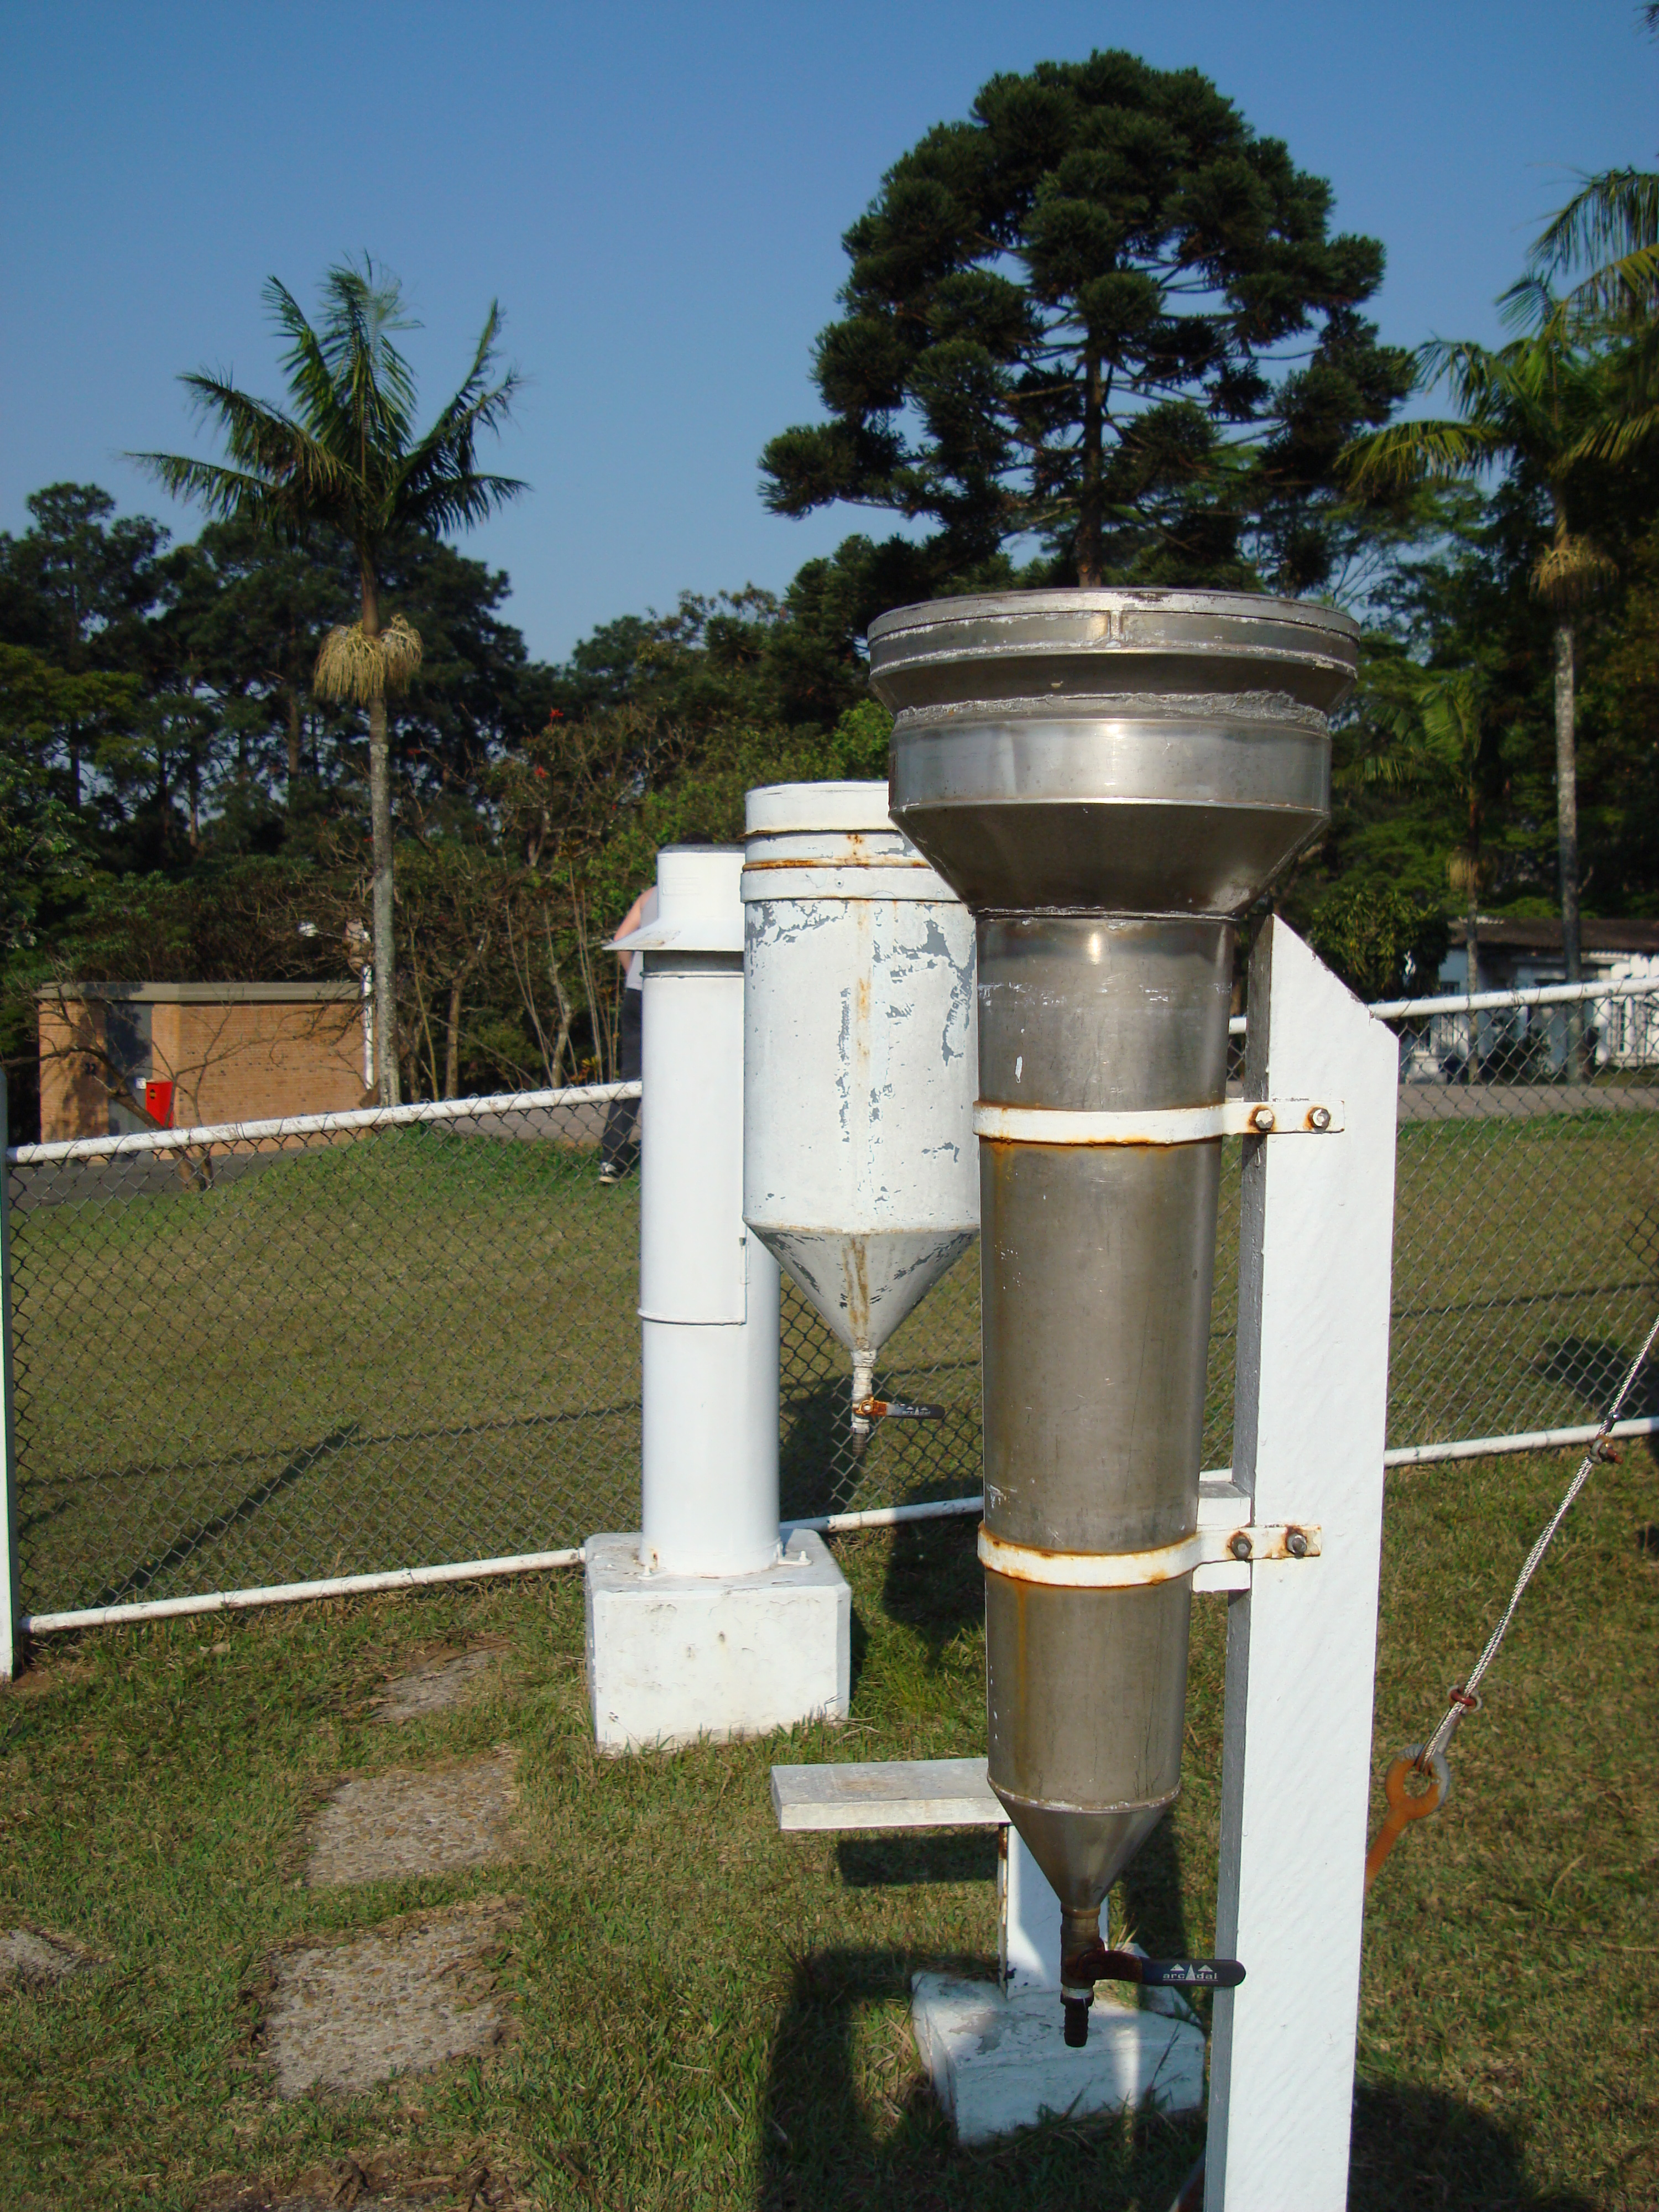
\includegraphics[width=0.5\textwidth]{Textuais/Figuras/pluviometro.jpg}
    \fonte{Autores}
    \label{fig:pluviometro}
\end{figure}

\subsection{Pluviógrafo}

Outro tipo de medidor de chuvas é o Pluviógrafo (Figura 2). Existe uma grande variedade de aparelhos, usando princípios diferentes para medir e gravar continuamente as chuvas. Os pluviógrafos permitem medir as intensidades das chuvas durante intervalos de tempo àqueles obtidos com as observações manuais feitas nos pluviômetros (TUCCI, 2004).

\begin{figure}
    \caption{Representação do pluviografo}
    \centering
    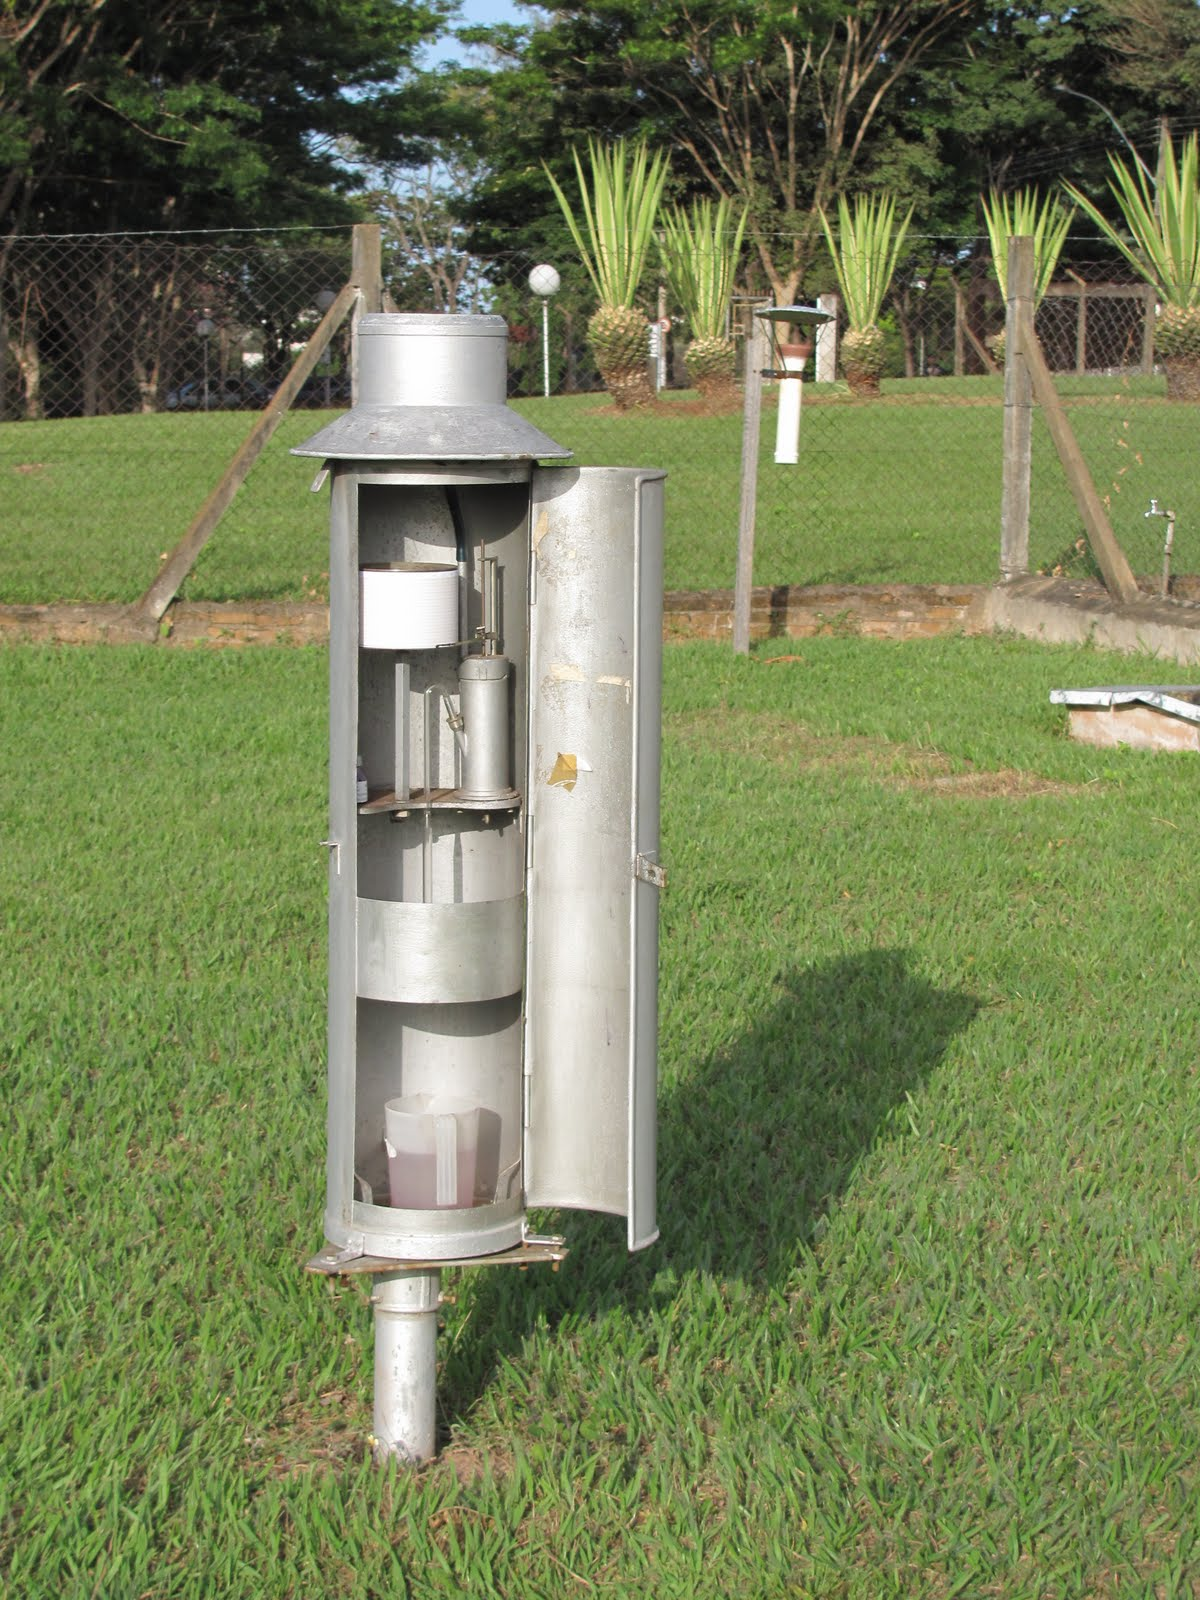
\includegraphics[width=0.5\textwidth]{Textuais/Figuras/pluviografo.jpg}
    \fonte{Autores}
    \label{fig:pluviografo}
\end{figure}

\section{Dados de chuvas no Brasil}

A Agência Nacional de Águas (ANA) disponibilizada uma relação dos postos pluviométricos instalados e operandos em todo o território brasileiro e os respectivos dados de chuva. Estas informações podem ser obtidas pela Internet por meio do Sistema de Informações Hidrológicas (HidroWeb). 

É importante destacar que, deve-se conhecer a qualidade dos dados que estão sendo utilizados, pois isso pode avariar a qualidade dos resultados dos estudos hidrológicos. Tratando-se de projetos em área urbana, recomenda-se que seja instalado ao menos um pluviógrafo, para aumentar a qualidade dos estudos hidrológicos que apoiarão, por exemplo, os projetos de controle de inundação (TUCCI, 1993).

\section{Caracterização das chuvas intensas}

A intensidade máxima média de precipitação cresce à medida que aumenta o período de retorno, sendo diretamente proporcionais, e decresce com o aumento da duração do evento, sendo inversamente proporcional a duração \cite{analise-chuva}. A principal forma de caracterização de chuvas intensas é por intermédio das equações de intensidade, duração e frequência da precipitação pluvial (equações IDF), ou equações de chuvas intensas \cite{tucci1993}, mais comumente representadas na forma da Equação \ref{eq:equacao-geral}. Estas equações são uma das ferramentas mais utilizadas nos trabalhos de engenharia relacionadas a recursos hídricos \cite{desagregacao}.

\begin{equation}
\label{eq:equacao-geral}
    i = \frac{k \times T_r^a}{(t+b)^c}
\end{equation}

Em que:

i = Intensidade máxima média de precipitação  $[mm.h^-1]$ 

$T_r$ = Período de retorno [anos]

t = Duração [min]

K, a, b, c = Parâmetros de ajuste estatístico, referentes à cada localidade

Para cada localidade ou plataforma de coleta de dados é feito, individualmente, o ajuste da equação para chuvas intensas. Recomenda-se ser feito com a utilização de um extenso período de dados, constituída de pluviógrafos \cite{interpolacao-chuva} apropriado a cada precipitação específica ocorrida em um posto pluviométrico, durante anos de observação. Entretanto, tais pluviógrafos dificilmente são disponíveis em quantidade e qualidade apropriada, devido à baixa densidade de equipamentos registradores espalhados no país, e às séries disponíveis serem frequentemente curtas e com falhas nos registros \cite{relacao-precipitacao}.

O estabelecimento de cada equação utiliza metodologia de exaustivo trabalho de tabulação, análise e interpretação de grande quantidade de pluviogramas, fitas utilizadas no registro por pluviógrafos \cite{relacao-precipitacao}. 

Decorrente da dificuldade de obtenção dos dados pluviográficos, a grande parte dos estudos realizados no Brasil, são efetuados com séries históricas inferiores à recomendada \cite{variabilidade-espacial}. A Organização Mundial de Meteorologia (OMM) recomenda a adoção de série histórica de no mínimo 30 anos.

Na prática, é difícil fixar o valor de intensidade da chuva, uma vez que o impacto é variável de local para local, seja em área rural ou urbana \cite{hidro-basica}. Em países subdesenvolvidos, as redes de dados climatológicos existentes são esparsas e escassas, reflexo na má qualidade dos projetos, originando obras sub ou superestimadas, quando superestimadas, podem gerar um desperdício econômico; e quando subestimadas, uma redução da confiabilidade de eficiência da obra e aumento do risco \cite{tucci1993}. Por esta razão, há barreiras na realização de projetos de obras hidráulicas mais confiáveis e econômicos \cite{chuva-bahia}. 

A busca por uma associação intensidade-duração-frequência de uma chuva é anterior a 1932 \cite{desagregacao}. Desde 1960 países desenvolvidos tem estudado a sua distribuição geográfica, onde possuem mapas que fornecem as intensidades e alturas de precipitação \cite{desagregacao}. Os estudos pioneiros no Brasil foram desenvolvidos por Pfafstetter (1957) e Denardin e Freitas (1982), em que Denardin e Freitas (1982) ajustaram equações matemáticas, a partir de gráficos apresentados por Pfafstetter (1957), que possibilitaram cálculo das alturas pluviométricas, em função da duração da precipitação e do período de retorno, por meio do método de regressão não-linear múltipla, para 80 estações pluviográficas distribuídas para todo o país \cite{relacao-idf-nordeste}.

No caso de não se ter informações provenientes de pluviogramas para determinar a equação de chuvas intensas, sendo a situação mais comum, existem alternativas para criação de informações das chuvas intensas \cite{interpolacao-chuva}. \citeonline{artigo-chuva} indicam a utilização de equações de regiões próximas, reduzindo a probabilidade de afetar a confiabilidade da estimativa. Outra alternativa bastante comum é a utilização de dados pluviométricos de captação diários, adquiridos de estação para estimar as equações, com a aplicação de métodos para desagregação de chuvas \cite{idf-rs}, o qual aproxima intensidades para durações inferiores a um dia \cite{relacoes-sc}. Finalmente, uma alternativa que vem ganhando espaço para a estimação dos parâmetros das equações de chuvas intensas em localidades sem qualquer registro de chuva consiste no uso de técnicas de interpolação espacial \cite{chuva-bahia}.

\begin{figure}[H]
    \caption{Representação das equações IDF}
    \centering
    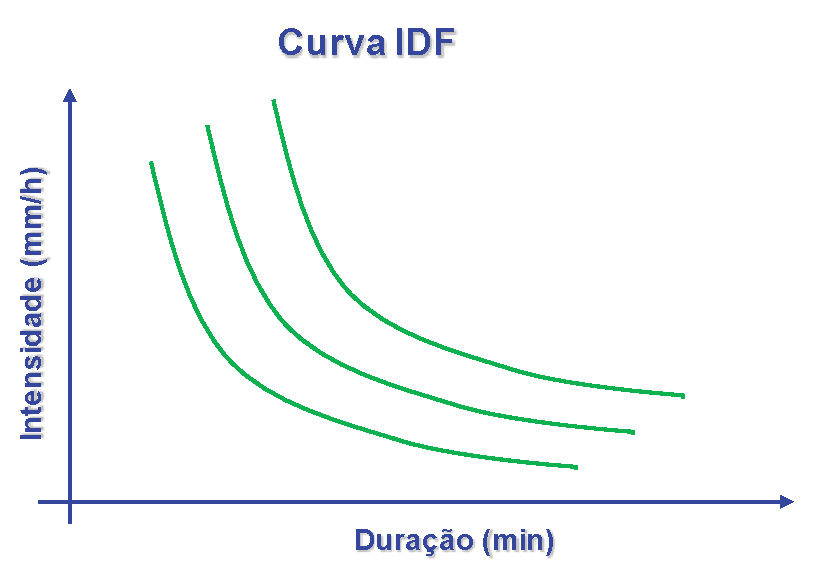
\includegraphics[width=0.8\textwidth]{Textuais/Figuras/curva-idf.pdf}
    \fonte{Autores}
    \label{fig:desagregacao}
\end{figure}

\section{Modelos matemáticos que expressam a relação IDF}

As relações intensidade-duração-frequência podem ser expressas matematicamente, ou seja, equações propostas que representam a quantidade máxima de uma chuva. A definição do modelo que representa as chuvas intensas, utilizado em cada trabalho, deve ser de fácil manuseio, mantendo a segurança em seus resultados que devem ser o mais próximo à realidade (MELLO, LIMA e MELLO, 2003).

Segundo Villela e Mattos (1975), o modelo matemático clássico mais utilizado é expresso pela Equação 1.

Em situações onde a escassez de dados é muito grande, (MELLO, LIMA e MELLO, 2003) evidenciam a importância da comparação entre vários modelos que representam a relação IDF, podendo resultar em informações confiáveis e precisas. Em seu trabalho, os autores, utilizam modelos exponencial e linear (Equação 2 e 3).

Mello et al. (2003) concluíram que o modelo exponencial produziu erros menores, gerando melhores aproximações da intensidade máxima de chuvas. O modelo linear, apesar de possuir um coeficiente de determinação $r^2$ superior a 0,99, não foi considerado confiável para utilização em estudos de chuvas intensas pois apresenta os maiores erros médios e, também, a maior amplitude de erros comparado ao modelo exponencial.

Pfafstetter (1957), em seu trabalho de determinação das curvas IDF, realizou o ajuste do modelo representado pela Equação 4.

A Equação 4 fornece a precipitação para período de retorno de 1 ano e a Equação 5 permite estimar a chuva para outros tempos de retorno (TUCCI, 2004).

Bertoni e Tucci (2001) detalharam a metodologia de Bell, que relaciona a precipitação máxima para um tempo de duração definido e período de retorno a uma precipitação padrão de 60 min de duração e 2 anos de período de retorno (Equação 6).

Se acordo com Sampaio (2011), a metodologia Bell se baseia em séries de chuva, observados em todo globo terrestre, destacando que o valor máximo das chuvas está relacionando a regiões convectivas com características parecidas no mundo todo; assinalando isso com uma desvantagem do método, uma vez que as equações são geradas de valores médias e não específicos para uma determinada região. O autor, também, apontou como desvantagem que o valor da precipitação máxima obtida é válido apenas para durações entre 5 a 120 min.
Mello et al. (2003) comentaram que a principal característica do método de Bell é o ajuste da equação, que pode ser regionalizada e que alguns autores optam pelo emprego do modelo de Bell, para o Brasil, atribuindo valores fixos aos parâmetros de ajuste, variando apenas o período de retorno e a intensidade da chuva.
    
Mello et al. (2003) realizaram ajustes do modelo de Bell para as seguintes regiões: Norte, Sul, Centro, Leste e Triângulo Mineiro e alcançaram um desvio inferior a 8\% entre os valores empíricos e teóricos.

O método de Bell mostra-se adequado para estimar as máximas precipitações de curta durações, sendo uma opção na determinação das chuvas críticas de projeto quando as séries disponíveis contém poucos anos de observação (Oliveira, Antonini e Griebeler 2008). Oliveira et al. (2011) aplicaram o modelo de Bell para PCD no Estado do Mato Grosso e verificaram que, comparado com as relações IDF elaboradas pelo modelo clássico (apresentado na Equação 1), o modelo de Bell superestimou a chuva de projeto.

Chen (1983) sugeriu uma equação IDF utilizando três alturas de precipitação: chuva com duração de 1 hora e período de retorno de 10 anos; chuva com duração de 24 horas e período de retorno de 10 anos; chuva com duração de 1 hora e período de retorno de 100 anos. De acordo com o autor, verificou-se que, nas precipitações a partir da duração de 2 horas, as relações de duração em relação à chuva de 24 horas variaram em função da relação da chuva de 1 hora e à de 24 horas. A Equação 7, proposta por (CHEN, 1983), foi desenvolvida para as séries anuais.

\section{Análise de frequência de séries históricas}

\subsection{Tipos de séries}

Os projetos de drenagem urbana são projetados com período de retorno de 5, 10 ou mais anos, em média. Por esse motivo, é necessário o conhecimento da frequência de ocorrência dos eventos extremos.

As relações entre intensidade, duração e frequência das chuvas intensas são inferidas das observações de precipitações de um grande período de observações, para que seja aceitável as frequências como probabilidades. Essas relações se efetuarão em curvas de intensidade-duração, uma para cada frequência, todas com caráter de regularidade (WILKEN, 1978).

\textit{Dois tipos de séries podem ser utilizados nas análises de frequências dos dados de chuva: as séries anuais que incluem a altura pluviométrica máxima de cada ano, e as séries parciais constituídas por alturas pluviométricas acima de um certo valor-base, independente do ano em que possam ocorrer (WILKEN, 1978).}

A escolha do tipo da série depende do tamanho da mesma e do objetivo do estudo. As séries parciais fornecem resultados mais consistentes para períodos de retorno inferiores a 5 anos, e números de anos de dados menores que 12 anos (TUCCI, 2004).

Além disso, as duas séries contemplam, praticamente, os mesmos resultados para períodos de returno superiores a 10 anos (DAEE, 2008).

\section{Desagregação de chuvas}

O método de desagregação de chuvas trata-se de uma metodologia com vantagem de uso simples, fornecendo resultados satisfatórios e com boa similaridade para locais distintos, além de permitir uma validade para regiões próximas onde não há medição. \citeonline{praticas-hidrologicas} desenvolveu a metodologia das isozonas, que pode ser aplicada em todo o território nacional. Dentro dos métodos mais utilizados, destacam-se os trabalhos de \citeonline{chuva-diaria} e \citeonline{idf-rs}, nos quais foram utilizadas séries de chuvas sintéticas para estimar as correlações de intensidade-duração-frequência, porém a metodologia mais utilizada é aquela que correlaciona a duração de chuvas com maiores durações para chuvas intensas de durações inferiores.

O método das isozonas foi comparado, pelos órgãos responsáveis pelas rodovias do Estado de Goiás e Departamento Nacional de Estradas e Rodagem, com as equações de chuvas intensas e encontraram desvios entre 7,0 e 55\%, sendo recomendada a busca por outra metodologia de cálculo \cite{isozonas}.

%explicar melhor esse parágrafo
Quanto ao método de desagregação de chuvas, podem ser encontradas na literatura diversas metodologias para obter durações de chuvas intensas de menores durações a partir de uma chuva de maior duração. Basicamente o método consiste em adotar um intervalo de maior precipitação em uma chuva de maior duração como a intensidade máxima para uma chuva de menor duração. A Figura \ref{fig:desagregacao} mostra como uma chuva de maior duração pode ser utilizada para estimar a máxima precipitação para chuvas de duração inferiores as coletadas.

\begin{figure}[h]
    \caption{Representação da metodologia de desagregação das chuvas}
    \centering
    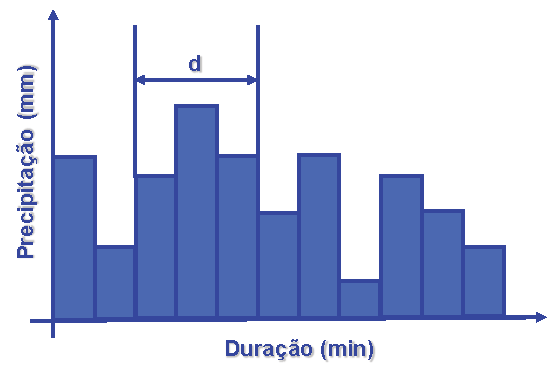
\includegraphics[width=0.7\textwidth]{Textuais/Figuras/desagregacao.pdf}
    \fonte{Autores}
    \label{fig:desagregacao}
\end{figure}

\subsection{Método de Damé (2001)}

Para \citeonline{dame01} foram utilizados os parâmetros do modelo Bartlett-Lewis do Pulso Retangular Modificado (BLPRM) \cite{iturbe} e, como consequência, as séries de chuvas na duração de 15 minutos foram separadas de uma chuva com duração de 24 horas e implementadas no modelo de desagregação proposto por \citeonline{point-process}.

O modelo BLPRM considera como hipótese que a precipitação tenha estacionalidade mensal, ou seja, que suas propriedades estatísticas (média, variância, covariância, probabilidade de ocorrência de períodos secos) não se alterem dentro do mês. No trabalho de \cite{chuva-diaria} o método das relações (MR) foi utilizado para obter uma curva IDF histórica obtida por meio de dados pluviográficos para o mesmo período de anos; os resultados mostram que a IDF obtida pelo MR representou adequadamente a IDF histórica, levando os autores concluírem que este método é eficaz na desagregação da chuva diária. Dessa forma, é viável a possibilidade de usar esse método para obter relações de intensidade-duração-frequência em regiões nas quais se tenha pouco ou nenhuma informação pluviográfica e que existam abundantes registros de chuva diária.

Assumindo de que o método das relações foi eficaz na separação de chuvas diárias e que forneceu resultados próximos aos que seriam obtidos por meio do uso de plataforma de coleta de dados, verificou-se o desempenho das estimativas dos valores de intensidades máximas, quando se utiliza o método das relações para desagregar a chuva diária e estimar as relações IDF e assim chegar a uma conclusão sobre o método das relações.

\subsection{Método de Bell (1969)}

\citeonline{bell} estabeleceu relações experimentais entre chuvas com diferentes durações fundamentado em informações de séries fracionais de chuva observada nos EUA, Austrália, URSS, Porto Rico, Alasca, África do Sul e Havaí. O fundamento teórico desse estudo é a existência de similaridade entre a formação de chuvas. Devido a propriedades semelhantes em muitas partes do mundo, devido a características de chuvas convectivas,  utiliza-se a equação de Bell para estimar a chuvas máximas entre os limites especificados. Devido aos valores adotados serem de várias regiões do mundo esses valores representam valores médios e não específicos de uma região; outra limitação está na durações das chuvas, que devem estar entre 5 minutos e 120 minutos; pode-se, também destacar, como limitação ao método de Bell, a obrigatoriedade de se conhecer a precipitação máxima com duração de 60 minutos e intervalo de retorno de 10 anos, sendo necessária a coleta de dados por meio de pluviógrafos.

\citeonline{bell} utilizou dados de vários continentes e ajustou a Equação \ref{eq:bell}.

\begin{equation}
\label{eq:bell}
    P_{(t,T)} = (0,21 \times Ln(T) + 0,52)(0,54\times t^{0,25} -0,5) \times P_{(1,10)}
\end{equation}

Em que:

$P_{(t,T)}$ = Altura de chuva [mm]

T = Período de retorno [anos]

t = Tempo de duração [min]

$P_{(1,10)}$ = Altura de chuva com 1 hora de duração e período de retorno de 10 anos


\subsection{Método de Chen (1983)}

\citeonline{rainfall} desenvolveu uma equação de IDF de chuvas que utiliza três alturas de precipitação: chuva de duração de 1 hora e tempo de retorno de 10 anos, chuva de 24 horas de duração e 10 anos de período de retorno e a chuva de 24 horas de duração e 100 anos de período de retorno. Neste estudo foi verificado que a partir da duração de 2 horas as relações de duração em relação a chuva de 24 horas variaram em função da relação da chuva de 1 hora e a de 24 horas.

A fórmula generalizada de \citeonline{rainfall} desenvolvida para as séries anuais, é dada pela Equação \ref{eq:chen1983}.

\begin{equation}
\label{eq:chen1983}
    P_{(t,T)} = \frac{a\times P(1,10)\times Log(10^{2-w}\times (Ln\frac{T_r}{T_r-1})^{1-w})}{(t+b)^c} \frac{t}{60}
\end{equation}

Em que:

P(t,T) = Altura de chuva com duração t e período de retorno $T_r$

$T_r$ = Período de Retorno [anos]

P(1,10) = Altura de chuva com 1 hora de duração e período de retorno de 10 anos

w = Relação entre a chuva de 1 hora de duração e período de retorno de 100 anos e a chuva de 1 hora de duração e período de retorno de 1 ano.

a, b,c = Obtidos em função da relação entre P(1,T) e P(24,T)


\section{Ajuste a distribuições estatísticas}

O desenvolvimento tecnológico e científico possibilita registrar o comportamento das variáveis hidrológicas, como por exemplo, chuvas, níveis de rios e nevascas. O acúmulo dos dados permitiu a criação de séries históricas, as quais são analisadas utilizando à estatística como uma ferramenta de tratamento de dados, dessa maneira o conhecimento dos conceitos estatísticos é indispensável ao desenvolvimento de estudos em hidrologia \cite{hidrologia-estatistica}.

\textit{As variáveis hidrológicas e hidrometerológicas têm sua variabilidade registrada por meio das chamadas séries temporais, as quais reúnem as observações ou medições daquela variável, organizadas de forma sequencial de sua ocorrência no tempo (ou espaço). Por limitações impostas pelos processos de medição ou observações, as variáveis hidrológicas, embora apresentem variações instantâneas são contínuas ao longo do tempo, ou do espaço, têm seus registros separados por determinados intervalos de tempo, ou de distância \cite{hidrologia-estatistica-np}.}

De acordo com \citeonline{hidrologia-estatistica-np} as séries hidrológicas podem incluir todas as observações disponíveis, coletadas em intervalos de tempo regulares ao longo de vários anos de registros, ou apenas alguns de seus valores característicos como, por exemplo, os máximos anuais ou as médias mensais. 

Com o ajuste de um modelo de chuva diária baseando-se nos estudos de \citeonline{relacao-precipitacao} é possível aumentar a eficiência dos dados de chuvas, principalmente por conseguir a simulação e criação de extensas séries de precipitação, sendo estas, muitas vezes, maiores que as próprias séries de dados observados.

No caso específico de eventos hidrológicos extremos, como por exemplo máximos e mínimos, as séries reduzidas podem ser anuais, quando os registros consecutivos possuem o mesmo intervalo no tempo, ou de duração segmentada, em caso contrário.

As séries de máximos valores são empregadas para ajuste, segundo a lei probabilística que melhor descreva o processo, possibilitando extrapolações \cite{spchuva}.

\textit{Distribuições teóricas de probabilidade são simplesmente funções analíticas usadas para descrever o comportamento de determinadas variáveis. No caso de extremos, só os ajustes das séries longas em múltiplas localidades é que dá indicações sobre as distribuições que levam a melhor extrapolação \cite{piracicaba}.}

Embora a teoria probabilística fundamental de valores extremos tenha sido desenvolvida há muito tempo, a modelagem estatística de extremos ainda permanece como assunto ativo de pesquisas dado seu importante papel nos projetos e gerenciamento de recursos hídricos, especialmente em um contexto de mudanças climáticas \cite{extremes}.

A teoria de valores extremos é fundamental nestes casos para a modelagem destes eventos. Os fundamentos desta teoria foram desenvolvidos por Fisher- Tippett (1928), que definiram os três tipos possíveis de distribuições assintóticas de valores extremos, conhecidas como de Gumbel (tipo I), Fréchet (tipo II) e Weibull (tipo III) \cite{ejgumbel}, que são casos especiais da Distribuição Generalizada de Valores Extremos desenvolvida por \citeonline{jen}. Além das distribuições de valores extremos, também são bastante utilizadas para descrever eventos raros as distribuições Log-normal e Pearson III \cite{sev}.

Diferentes distribuições, escolhidas entre as mais frequentemente utilizadas na descrição destas variáveis são consideradas, incluindo a de Gumbel, Log-Normal, Pearson III, Fréchet e Weibull, que tem, respectivamente, como funções de densidade de probabilidade acumulada.

\subsection{Distribuição de Gumbel}

Em geral, as distribuições de valores extremos de grandezas hidrológicas ajustam-se adequadamente à distribuição de Fisher- Tippett do tipo I, também nomeada como função de Gumbel \cite{hidro-aplicada}.

A distribuição de probabilidade de Gumbel é aplicada às séries históricas de valores extremos, especialmente, a precipitação máxima diária anual, sendo expressa pela Equação \ref{eq:gumbel}.

\begin{equation}
\label{eq:gumbel}
    P = 1 - e^{-e^{\gamma \times T_r}}
\end{equation}

A variável reduzida da distribuição de Gumbel é obtida pela aplicação da função de distribuição de frequência de Chow.

\begin{equation}
    \gamma_{Tr} = - Ln^{-Ln \left( 1 - \frac{1}{T_r} \right)}
\end{equation}

O evento extremo $X_Tr$ é representado pela Equação \ref{eq:evento-extremo}.

\begin{equation}
\label{eq:evento-extremo}
    X_{Tr} = \overline{x} + k_{Tr} \times s
\end{equation}

Em que:

$\overline{x}$ = Média dos valores extremos da série histórica

s = Desvio padrão amostral

$X_{Tr}$ = Evento extremo no decorrer do ano

\subsection{Distribuição de Fréchet}

A distribuição de Fréchet é uma forma particular da distribuição de valores extremos do Tipo II e de acordo com \citeonline{hidrologia-estatistica-np}, essa distribuição é conhecida também pela denominação Log-Gumbel, sendo pela Equação \ref{eq:frechet}.

\begin{equation}
\label{eq:frechet}
    P(x) = e^{-e^{-\alpha(x-\beta)}}
\end{equation}

\textit{No caso dos valores máximos, a distribuição de Fréchet refere-se à forma assintótica limite para um conjunto de N variáveis aleatórias originais, independentes e igualmente distribuídas conforme um modelo, de cauda superior polinomial. A distribuição foi usada pela primeira vez na análise de frequência de vazões de enchentes por Fréchet (1927), tendo, desde então, encontrado aplicações, como distribuição extrema de eventos hidrológicos máximos.}

\subsection{Distribuição de Weibull}

Segundo \citeonline{catalunha} a distribuição de Weibull é utilizada em análise hidrológica para eventos extremos, sendo pouco conhecida a sua utilização em séries climáticas. Tem como principal método de ajuste de distribuição o da máxima verossimilhança, que consiste em determinar os valores de g e b pelas suas equações fundamentais.

A distribuição de Weibull a dois parâmetros tem como função de distribuição de probabilidades acumulada (FDA) a Equação \ref{eq:weibull}.

\begin{equation}
\label{eq:weibull}
    P(x) = 1 - e^{-(\frac{x-\alpha}{\beta})^\lambda}
\end{equation}

\citeonline{catalunha} realizou um trabalho em Minas Gerais, concluindo que a distribuição de Weibull possui um ótimo desempenho para estimar as precipitações diárias.

\citeonline{chuvas-brasil}, realizando os primeiros estudos no Brasil, utilizou séries de valores extremos de precipitações de 98 plataformas de coleta de dados distribuídas em várias regiões do Brasil, para a construção de curvas IDF, utilizando com ferramenta estatística a distribuição de Weibull.

\subsection{Distribuição Log-Normal}

A distribuição Log-Normal tem como função de distribuição de probabilidades acumulada (FDA) a Equação \ref{eq:lognormal}.

\begin{equation}
\label{eq:lognormal}
    P(x) = \frac{1}{(x-a) \times \sqrt{2\pi\sigma^2}} \int_{-\infty}^{\infty} e^{-0,5} \left( \frac{Ln(x-a)-\mu}{\sigma^2} \right) dx
\end{equation}

A distribuição Log-Normal mostrou-se adequada para previsão das chuvas prováveis apenas nos meses de maiores intensidades segundo \citeonline{lavras}.

\section{Teste de Aderência}

De acordo com \citeonline{oliveira}, a grande dificuldade com o desenvolvimento de modelos hidrológicos é a validação dos resultados obtidos, onde se deseja determinar indícios documentados que provem um alto grau de garantia a um processo específico, assegurando constantemente que os resultados estejam de acordo com a distribuição presentada para o conjunto de dados.

Diversos procedimentos estatísticos convencionais têm sido usados para este fim, tais como teste de comparação de médias (teste t), testes de comparação de variâncias (desvio padrão) como teste F, intervalos de confiança e outros diferentes níveis de probabilidade, e para a comparação de frequências de dados agrupados são normalmente utilizados os testes $X^2$ e Kolmogorov-Smirnov \cite{oliveira}.

O mesmo autor afirma que quando se ajusta uma distribuição de probabilidade a um conjunto de dados, trabalha- se com a hipótese de que a distribuição representa adequadamente aquele conjunto de informações.

Assim, \citeonline{climatologia}, comentam que em trabalhos de hidrologia, para se julgar a adequação do ajustamento dos dados observados a distribuição de frequência os testes estatísticos qui- quadrado ($x^2$) e o de Kolmogorov- Smirnov tem apresentado os melhores resultados.

\subsection{Qui-Quadrado}

O teste do $\chi^2$ é aplicado para verificar o ajuste de distribuição de probabilidade conhecida, no caso a gama, a uma amostra de dados de uma distribuição de probabilidade desconhecida. No teste do $\chi^2$ , a hipótese de nulidade admite que as frequências observadas se ajustem as frequências calculadas com a distribuição teórica (gama, exponencial, normal, Weibull) com seus parâmetros estimados com base nos dados amostrais. O valor de $\chi^2$ é dado pela Equação \ref{eq:chiquadrado}.

\begin{equation}[h]
\label{eq:chiquadrado}
    \chi^2=\sum_{i=1}^{k} \frac{(F_{0i}-F_{ei})^2}{F_{ei}}
\end{equation}

Se o valor do $\chi^2$  calculado é menor que o $x^2 1 - a$, k- p - 1 , sendo esse último proveniente de uma distribuição com GL = k – p - 1 graus de liberdade, sendo p o número de parâmetros estimados com base nos dados (p = 2, para o caso da distribuição gama) e a é o nível de significância estabelecido à hipótese de nulidade não é rejeitada e pode- se afirmar que os dados amostrais se aderem à distribuição teórica com um nível de significância a.

\citeonline{catalunha} em seu trabalho realizado em Minas Gerais aplicando cinco funções de densidade de probabilidade a séries de precipitação, concluíram que o teste do $x^2$  apresentou melhores características para verificar o ajuste de uma distribuição de probabilidade estimada a dados observados.

\begin{figure}[h]
    \caption{Representação do qui quadrado}
    \centering
    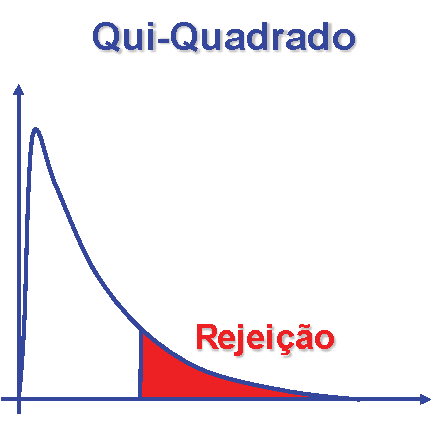
\includegraphics[width=0.5\textwidth]{Textuais/Figuras/qui-quadrado.pdf}
    \fonte{Autores}
    \label{fig:qui-quadrado}
\end{figure}

\subsection{Kolmogorov-Smirnov}

Esse teste é aplicado para verificar se os valores de uma certa amostra de dados podem ser considerados de uma população, com distribuição teórica pré-estabelecida.
\citeonline{rio-paraiba} utilizaram o teste de aderência de Kolmogorov- Smirnov a um nível de 5\% de probabilidade para verificar se o ajuste dos dados pluviométricos mensais se ajustam a função de distribuição de probabilidade normal e gama mista. O teste relaciona duas distribuições de frequências acumuladas, uma F’(x) teórica e outra F(x) derivada dos dados amostrais. O valor de Dmax é pela Equação \ref{eq:kolmogorov}.

\begin{equation}
\label{eq:kolmogorov}
    D_{Max} = Max|F'(x) - F(x)|
\end{equation}

Caso o valor do Dmax observado é inferior ao Dmax obtido em tabelas, a um determinado nível de significância $\alpha$ , a hipótese de nulidade não é rejeitada, dessa forma, pode-se afirmar que os dados amostrais tem aderência à distribuição teórica.

\begin{figure}[h]
    \caption{Representação kolmogorov}
    \centering
    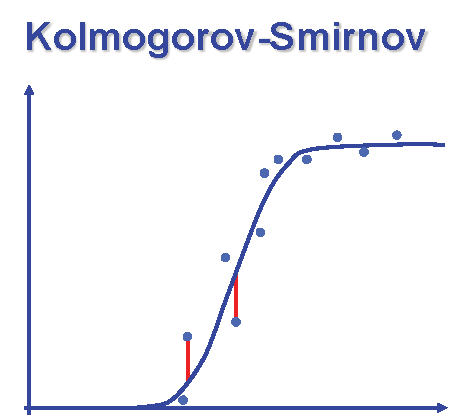
\includegraphics[width=0.5\textwidth]{Textuais/Figuras/kolmogorov.pdf}
    \fonte{Autores}
    \label{fig:kolmogorov}
\end{figure}

\section{Inteligência Artificial}

O termo aprendizado de máquina refere-se à detecção automatizada de padrões significantes em dados. Nas últimas décadas tem se tornado uma ferramenta comum em quase qualquer tarefa que requer informações extraídas de uma grande quantidade de dados (SHWARTZ e DAVID, 2014).

A ciência do aprendizado tem um importante papel em áreas como a estatística, mineração de dados e inteligência artificial, passando por áreas como engenharia, medicina, astronomia, robótica e outras disciplinas (HASTIE, TIBSHIRANI e FRIEDMAN, 2008).

Com o contínuo aumento de informações em forma digital, a necessidade de métodos automatizados para análise de dados continua crescendo. O objetivo do aprendizado de máquina é desenvolver métodos que possibilitam a detecção de padrões em dados, para futuramente reutilizá-los em forma de previsões em novos dados. (MURPHY, 2012)

Dentre as ferramentas que integram a inteligência artificial destacam-se os Algoritmos Genéticos, Lógica Difusa e Redes Neurais Artificiais (FILIPATTI, et al., 2000), sendo que este trabalho será focado em Redes Neurais Artificiais (RNA).

\section{Tipos de aprendizado}

Os sistemas de aprendizado de máquina possuem características peculiares que possibilitam uma classificação não exclusiva desses sistemas em função da linguagem de descrição, modo de aprendizado, paradigma de aprendizado, formas e tarefa de aprendizado.
O aprendizado depende da interação entre o ambiente e aprendiz. A primeira diferença consiste no aprendizado supervisionado e não supervisionado \cite{uml}.

\subsection{Aprendizado supervisionado}

O aprendizado supervisionado é aquele cujos parâmetros são pré-definidos e o algoritmo procura um padrão entre os dados. As informações que serão utilizadas para treinamento já contêm informações suficientes que permitem o algoritmo inferir uma relação entre uma ou múltiplas variáveis. A característica básica de sistemas de aprendizado supervisionado é de que os dados que são utilizados para treiná-los contém a resposta desejada, isto é, contém a variável dependente resultante das variáveis independentes observadas. Nesse caso, alega-se que os dados são anotados com as respostas ou classes a serem previstas \cite{learning-algorithms}.

De acordo com \citeonline{learning-algorithms} as técnicas mais usuais para resolver problemas de aprendizado supervisionado são: regressão linear, regressão logística, redes neurais artificiais, máquina de suporte vetorial (ou máquinas kernel), árvores de decisão, k-vizinhos mais próximos e Bayes ingênuo. Aprendizado de máquina supervisionado é a área que concentra a maioria das aplicações bem sucedidas e onde a grande parte dos problemas já estão bem definidos.

A Figura \ref{fig:reg-linear} representa um exemplo de aprendizado supervisionado, a regressão linear.

\begin{figure}[h]
    \caption{Regressão linear é um exemplo de aprendizado supervisionado}
    \centering
    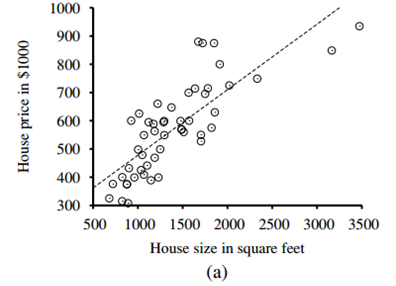
\includegraphics[width=0.8\textwidth]{Textuais/Figuras/linear-ml.png}
    \fonte{\citeonline{ai}}
    \label{fig:reg-linear}
\end{figure}

\subsection{Aprendizado não-supervisionado}

O aprendizado não supervisionado, permite abordar problemas com pouca ou nenhuma ideia de como deverá ser o resultado. A rede tem de descobrir relações, padrões, regularidades ou categorias nos dados que lhe vão sendo apresentados e codificá-las em saídas. Em alguns casos, conseguir dados anotados é extremamente custoso ou até mesmo impossível. De uma forma geral, com aprendizado não supervisionado pretende-se achar uma representação mais informativa dos dados que temos. Geralmente, essa representação mais informativa é também mais simples, condensando a informação em pontos mais relevantes \cite{ai}.

A Figura \ref{fig:nao-supervisionado} exemplifica o aprendizado não supervisionado: a classificação de dados em dois grupos.

\begin{figure}[h]
    \caption{(a) Distribuição da altura e peso de algumas pessoas. (b) Possível agrupamento de dados em 2 grupos}
    \centering
    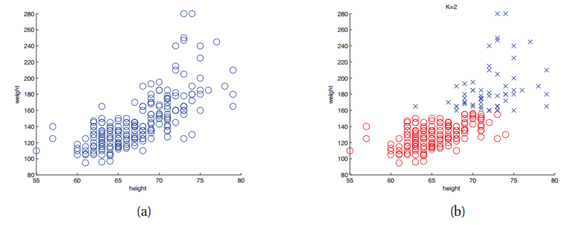
\includegraphics[width=1.0\textwidth]{Textuais/Figuras/nao-supervisionado.png}
    \fonte{Murphy (2012)}
    \label{fig:nao-supervisionado}
\end{figure}

\subsection{Benefícios das RNA}

O poder de abstração das RNA deve-se à sua estrutura paralela e à capacidade de aprendizagem \cite{big-data}. A estrutura paralela resulta da existência de muitos neurônios ligados em uma mesma estrutura de pesos de conexão com facilidade de adaptação a distintos tipos de entrada de dados. A estrutura paralela é desejável uma vez que permite a tolerância à falha, pois se algum neurônio falhar, os efeitos na rede como um todo não serão significativos para o desempenho da rede, dado que existe outro caminho de ligação entre os nós que pode iludir a falha \cite{statistical-learning}.

Uma das principais características das RNA é a capacidade de aprender por meio de exemplos e de generalização, ou seja, reconhecer padrões em elementos que não foram apresentados antes, possibilitando a produção de resultado aceitável oriundo de uma nova entrada de informação \cite{neural-network}.

As principais propriedades que podem se destacar das redes neurais artificiais são: não linearidade, mapeamento de entrada e saída, adaptabilidade e tolerância a falhas \cite{neural-network}.

\subsection{Redes Neurais Artificiais}

Redes neurais artificiais foram originalmente planejadas no meio do século 20 como um modelo computacional do cérebro humano. Sua aplicação era limitada devido a limitação computacional disponível na época, além de algumas questões teóricas que não foram solucionadas por várias décadas \cite{mlpp}.

É teorizado que devido à sua inspiração biológica, algoritmos baseados em redes neurais artificiais serão capazes de simular como o ser humano reconhece conceitos e objetos \cite{learning-algorithms}.

Em uma análise matemática, as RNA podem ser explicadas como um mapeamento não linear de um vetor de espaço de entrada para um vetor de espaço de saída, que pode ser realizado por meio de camadas de funções de ativação, em que coordenadas de entrada são somadas de acordo com o valor de seus respectivos pesos e bias  para produzir uma saída simples, ativada ou não, de acordo com o respectivo nível de acionamento \cite{two-phase-flow}.

O conceito de rede neural artificial é basicamente introduzido pela biologia onde a rede neural tem um importante papel no ser humano. No corpo humano todo trabalho é realizado com ajuda da rede neural. Uma rede neural é uma cadeia de milhões de neurônios interconectados \cite{ann}, exemplificado pela Figura \ref{fig:neuronios}.

\begin{figure}[h]
    \caption{Neurônios humanos conectados entre si}
    \centering
    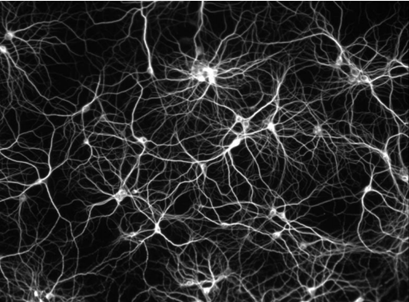
\includegraphics[width=0.55\textwidth]{Textuais/Figuras/neuronios.png}
    \fonte{Autores}
    \label{fig:neuronios}
\end{figure}

A terminologia rede neural é inspirada pelas operações biológicas realizadas por células especiais denominadas neurônios, mostrados na Figura \ref{fig:celula}. Um neurônio é uma célula biológica especial que processa informação de um neurônio para outro com ajuda de um impulso elétrico e mudanças químicas que ocorrem no cérebro. Todo o processo de receber e enviar informação é realizado de uma forma particular: um neurônio recebe informações de outro neurônio através dos dendritos e envia informações com picos de atividade elétrica através de um longo e fino suporte conhecido como axônio que os divide em sinapses para enviá-los para outros neurônios \cite{ai}.

\begin{figure}[h]
    \caption{Nomenclatura das partes que compõem um neurônio humano}
    \centering
    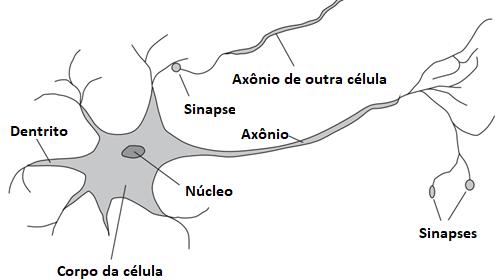
\includegraphics[width=0.8\textwidth]{Textuais/Figuras/celula.png}
    \fonte{https://news.psu.edu/story/441320/2016/12/08/research/how-make-motor-neuron}
    \label{fig:celula}
\end{figure}

As redes neurais artificiais têm o seu equivalente ao neurônio denominado nó que recebe um conjunto de entradas ponderadas, processa a sua soma com as funções de ativação $\phi$, e passa o resultado da função de ativação para o próximo nó até o término da rede (Equação \ref{eq:no}) \cite{ann}.

\begin{equation}
\label{eq:no}
    \phi \left( \sum_{i} w_i\times a_i \right) = \phi(w^T\times a)
\end{equation}

Visualmente é equivalente a Figura \ref{fig:neuronio-rna}.

\begin{figure}[h]
    \caption{Representação de um neurônio na RNA}
    \centering
    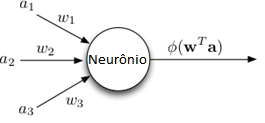
\includegraphics[width=0.31\textwidth]{Textuais/Figuras/rep-neronio.png}
    \fonte{http://briandolhansky.com/blog/artificial-neural-networks-linear-regression-part-1}
    \label{fig:neuronio-rna}
\end{figure}

\subsection{Funções de ativação}

Funções de ativação são basicamente funções de transferência que são geradas pelos neurônios artificiais e enviam sinais para outro neurônio artificial \cite{ann}. As funções de ativação mais comuns são: Limiar, Degrau, Degrau Unitário, Linear e Logística. A Figura \ref{fig:funcao-ativacao} ilustra essas funções. 

\begin{figure}[h]
    \caption{Funções de ativação}
    \centering
    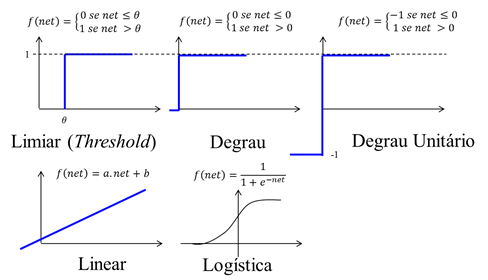
\includegraphics[width=0.8\textwidth]{Textuais/Figuras/funcao-ativacao.png}
    \fonte{https://pt.stackoverflow.com/questions/61187/como-implementar-a-camada-oculta-em-uma-rede-neural-de-reconhecimento-de-caracte}
    \label{fig:funcao-ativacao}
\end{figure}

A função de ativação linear é a função mais básica porque não altera a saída de um neurônio. Geralmente é utilizada nas camadas de saída em redes neurais de regressão. A Equação \ref{eq:linear}, mostra a função linear que também é denominada função identidade \cite{ai}.

\begin{equation}
\label{eq:linear}
    \phi(w^Ta) =w^Ta
\end{equation}

A função sigmoide (Logística) era a mais utilizada em RNAs, por serem biologicamente mais plausíveis. Como neurônios biológicos funcionam de forma binária (ativando vs não ativando), a função sigmoide é uma boa forma de modelar esse comportamento, já que assume valores apenas entre 0 (não ativação) e 1 (ativação). No entanto, observando sua derivada, pode-se ver que ela satura para valores acima de 5 e abaixo de -5. Com essas derivadas tendendo a zero, a propagação do gradiente desvanece nessas regiões, causando dificuldades no treinamento. A função logística é representada pela Equação \ref{eq:sigmoid} \cite{ai}.

\begin{equation}
\label{eq:sigmoid}
    \phi(w^Ta)=\frac{1}{1+exp(-w^Ta)} 
\end{equation}

Similar à função logística, a função Tangente Hiperbólica (tanh) também tem um formato de S, mas varia de -1 a 1, em vez de 0 a 1 como na logística. A tanh se aproxima mais da identidade, sendo assim uma alternativa mais atraente do que a sigmoide para servir de ativação às camadas ocultas das RNAs \cite{ai}.

\begin{equation}
\label{eq:tanh}
    \phi(w^Ta) = tanh(w^Ta)
\end{equation}

A possível criação de uma rede neural ocorre por meio do encadeamento dos nós. Usualmente esse processo é realizado utilizando camadas, as saídas de um nó estão conectadas a entrada dos nós da próxima camada \cite{tensor-flow}.

O objetivo de aproximações de funções é treinar uma rede neural que seja capaz, a partir de um conjunto de dados entrada-saída, de mapear uma determinada relação funcional que contemple o universo de amostras sob análise. O treinamento, nesse caso, envolve o aprendizado dos pesos de borda corretos para produzir a saída de destino, dada uma entrada \cite{uml}. A rede e seus pesos treinados formam uma função (denominada h) que operam sob dados de entrada. Com a rede treinada, é possível produzir previsões para valores de entrada previamente desconhecidos.

\begin{figure}[h]
    \caption{Exemplo de uma regressão e classificação}
    \centering
    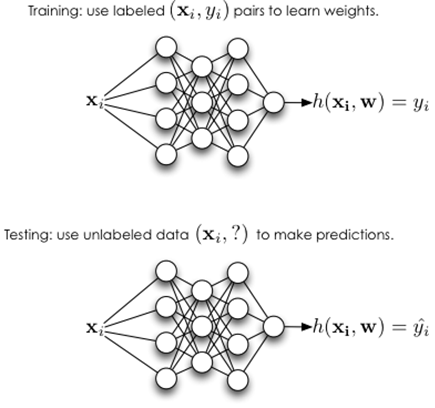
\includegraphics[width=0.7\textwidth]{Textuais/Figuras/rede-neural.png}
    \fonte{https://towardsdatascience.com/how-to-build-your-own-neural-network-from-scratch-in-python-68998a08e4f6}
    \label{fig:reg-class}
\end{figure}

É possível treinar uma rede neural para realizar regressão ou classificação. Nesse trabalho iremos abordar somente a regressão linear. 

\subsection{Regressão Linear}

Regressão linear é a forma mais simples de regressão \cite{ai}. Modelam-se o sistema como combinações lineares de entradas para produzir uma saída.

\begin{equation}
    y_i = h(x_i,w) = w^Tx_i
\end{equation}

A RNA torna-se responsável por encontrar os pesos que geram o melhor resultado para os dados de treinamento. Um modo de verificar a qualidade da aproximação é utilizando o método dos mínimos quadrados (também conhecido como \textit{Loss}) \cite{ltflow}.

\begin{equation}
    L(w) = \sum_i \left( h(x_i,w)-y_i^2 \right)^2
\end{equation}

Para poder realizar o melhor ajuste é preciso minimizar o valor de $L(w)$. Esse método possui uma solução analítica, mas em geral pode-se resolver utilizando o método do gradiente descendente \cite{ai}.

A rede neural mais simples utiliza o método dos mínimos quadrados para realizar uma regressão linear como mostra a Figura \ref{fig:linear}. 

\begin{figure}[h]
    \caption{Neurônio artificial e a saída gerada utilizando uma função linear de ativação}
    \centering
    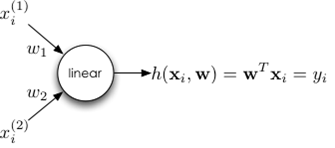
\includegraphics[width=0.45\textwidth]{Textuais/Figuras/linear.png}
    \fonte{http://briandolhansky.com/blog/artificial-neural-networks-linear-regression-part-1}
    \label{fig:linear}
\end{figure}

Essa rede recebe como entrada de dados, duas entradas $x_i^{(1)}$ e $x_i^{(2)}$, os pesos das entradas como $w_1$ e $w_2$ e os soma, e como saída tem-se a previsão $y_i$. Pode-se considerar uma rede neural com n parâmetros de entrada, porém a rede deve conter n pesos, sendo equivalente um peso para cada entrada. Para poder determinar a qualidade de aproximação é possível utilizar o método dos mínimos quadrados \cite{ML}.

\citeonline{tensor-flow} utiliza o método do gradiente descendente para minimizar os erros em relação aos dados de treinamento. Primeiramente deriva-se o gradiente descendente em relação a um determinado peso $w_{j \rightarrow k}$

\begin{equation}
    \frac{\partial}{\partial w_{j \rightarrow k}}L(w) = \frac{\partial}{\partial w_{j \rightarrow k}} \sum_i \left( h(x_i,w)-y_i^2 \right)
\end{equation}

\begin{equation}
    \frac{\partial}{\partial w_{j \rightarrow k}}L(w) = \sum_i \frac{\partial}{\partial w_{j \rightarrow k}} \left( h(x_i,w)-y_i^2 \right)
\end{equation}

\begin{equation}
    \frac{\partial}{\partial w_{j \rightarrow k}}L(w) = \sum_i 2(h(x_i,w)-y_i) \frac{\partial}{\partial w_{j \rightarrow k}} h(x_i,w)
\end{equation}

Nesse ponto, calcula-se o gradiente da função da rede em relação ao peso da derivada parcial. 

A função da rede é dada pela Equação \ref{eq:funcao-rede}.

\begin{equation}
\label{eq:funcao-rede}
    h(x_i,w) = w_1x_i^{(1)} + w_2x_i^{(2)}
\end{equation}

O gradiente em relação a $w_1$ é apenas $x_1$, e o gradiente em relação a $w_2$ é apenas $x_2$, dessa forma o gradiente é dado pela Equação \ref{eq:gradiente}.

\begin{equation}
\label{eq:gradiente}
    \nabla_wL(w) = \left( \frac{\partial L(w)}{\partial w_1}, \frac{\partial L(w)}{\partial w_2} \right) = \left( \sum_i 2x_i ^{(1)} h(x_i,w), \sum_i 2x_i ^{(2)} h(x_i,w) \right)
\end{equation}

Agora é possível atualizar os pesos utilizando o gradiente descendente padrão

\begin{equation}
    w = w -\eta \nabla_w L(w)
\end{equation}

Onde ``$\eta$`` é o passo.

\subsection{Treinamento da RNA}

Nesta fase, seguindo o algoritmo de treinamento escolhido, serão ajustados os pesos das conexões. É importante considerar, nesta fase, alguns aspectos tais como a inicialização da rede, o modo de treinamento e o tempo de treinamento \cite{aplicacao}.

Uma boa escolha dos valores iniciais dos pesos da rede pode diminuir o tempo necessário para o treinamento. Normalmente, os valores iniciais dos pesos da rede são números aleatórios uniformemente distribuídos, em um intervalo definido. A escolha errada destes pesos pode levar a uma saturação prematura. \citeonline{treinamento} encontraram uma função que pode ser utilizada para determinar valores iniciais melhores que valores puramente aleatórios \cite{aplicacao}.

Quanto ao modo de treinamento, na prática é mais utilizado o modo padrão devido ao menor armazenamento de dados, além de ser menos suscetível ao problema de mínimos locais, devido à pesquisa de natureza estocástica que realiza. Por outro lado, no modo batch se tem uma melhor estimativa do vetor gradiente, o que torna o treinamento mais estável. A eficiência relativa dos dois modos de treinamento depende do problema que está sendo tratado \cite{aplicacao}.

Quanto ao tempo de treinamento, vários fatores podem influenciar a sua duração, porém sempre será necessário utilizar algum critério de parada. O critério de parada do algoritmo recorrente não é bem definido, e geralmente é utilizado um número máximo de ciclos. Mas, devem ser considerados a taxa de erro médio por ciclo, e a capacidade de generalização da rede. Pode ocorrer que em um determinado instante do treinamento a generalização comece a degenerar, causando o problema de \textit{over-training}, ou seja a rede se especializa no conjunto de dados do treinamento e perde a capacidade de generalização \cite{aplicacao}.

O treinamento deve ser interrompido quando a rede apresentar uma boa capacidade de generalização e quando a taxa de erro for suficientemente pequena, ou seja menor que um erro admissível. Assim, deve-se encontrar um ponto ótimo de parada com erro mínimo e capacidade de generalização máxima \cite{aplicacao}.

\subsection{Testando a RNA}

Durante esta fase o conjunto de teste é utilizado para determinar a performance da rede com dados que não foram previamente utilizados. A performance da rede, medida nesta fase, é uma boa indicação de sua performance real.

Devem ser considerados ainda outros testes como análise do comportamento da rede utilizando entradas especiais e análise dos pesos atuais da rede, pois se existirem valores muito pequenos, as conexões associadas podem ser consideradas insignificantes e assim serem eliminadas (\textit{prunning}). De modo inverso, valores substantivamente maiores que os outros poderiam indicar que houve \textit{over-training} da rede.

Com a rede treinada, testar consiste em obter a previsão para cada ponto $x_i$ utilizando a função $h(x_i, w)$. O erro pode ser calculado da mesma forma do treinamento utilizando a Equação \ref{eq:teste-rna}.

\begin{equation}
\label{eq:teste-rna}
    L(w) = (\overline{y_i} - y_i)^2
\end{equation}

\subsection{Redes Neurais Recorrentes}

Diferentemente das redes neurais \textit{feed-forward}, redes neurais recorrentes possuem ciclos entre seus neurônios. Em outras palavras, neurônios podem ter conexões com neurônios de camadas anteriores, ou da mesma camada como mostra a Figura \ref{fig:recorrente}.

\begin{figure}[h]
    \caption{Exemplo de uma rede neural recorrente}
    \centering
    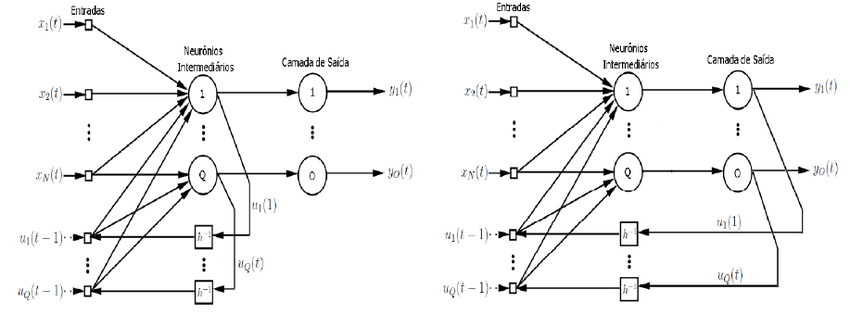
\includegraphics[width=0.9\textwidth]{Textuais/Figuras/recorrente.png}
    \fonte{https://goo.gl/wH6xmR}
    \label{fig:recorrente}
\end{figure}

Desta forma, a informação não flui em um único sentido, e a saída da rede não depende mais apenas da entrada corrente, mas também das entradas anteriores. O efeito prático disto é a existência de memória de curto prazo na rede.

Considerando o aprendizado por treinamento uma espécie de memória de longo prazo, então adicionalmente à nova capacidade de manter uma memória recente, redes neurais recorrentes podem criar modelos muito mais complexos, que apesar de serem de compreensão mais difícil apresentam capacidade de resolver uma gama maior de problemas \cite{rede-recorrente}.

Mesmo com redes neurais \textit{feed-forward} é possível ter um efeito similar ao de memória, como por exemplo, adicionando à entrada dados de entradas anteriores, multiplicando a dimensionalidade, ou mesmo adicionando parâmetros com algum aspecto temporal. Mas esses casos podem acabar causando o problema de maldição da dimensionalidade (\textit{curse of dimensionality}) onde a entrada fica muito complexa e dificulta o aprendizado e generalização \cite{rede-recorrente}.

Contudo, mesmo redes neurais recorrentes podem apresentar desafios no processo de treinamento. Ainda que na teoria sejam capazes de lidar com dependências de longo termo (longas sequências), Bengio et al. (1994) mostram através de experimentos que na prática isso muitas vezes não é possível, pois em métodos de treinamento baseados em gradientes a informação de erro desaparece \cite{rede-recorrente}.

\subsubsection{Limitações de redes recorrentes}

As redes neurais que utilizam recorrência, assim como muitos outros tipos de redes neurais artificiais, podem ser vistas como ``caixas pretas``, na qual quase não se sabe porque a rede chega a uma determinada saída, uma vez que os modelos não apresentam justificativas para suas respostas. Neste sentido, muitas pesquisas vêm sendo realizadas visando a extração de conhecimento de redes neurais artificiais, e na criação de procedimentos explicativos, onde se tenta justificar o comportamento da rede em determinadas situações  \cite{aplicacao}.

Uma outra limitação refere-se ao tempo de treinamento de redes neurais utilizando recorrência, que tende a ser muito lento. Algumas vezes são necessários milhares de ciclos para se chegar à níveis de erros aceitáveis, principalmente se estiver sendo simulado em computadores seriais, pois a CPU deve calcular as funções para cada unidade e suas conexões separadamente, o que pode ser problemático em redes muito grandes, ou com grande quantidade de dados \cite{aplicacao}.

É muito difícil definir a arquitetura ideal da rede de forma que ela seja tão grande quanto o necessário para conseguir obter as representações necessárias, ao mesmo tempo compacta o suficiente para se ter um treinamento mais acelerado. Não existem regras claras para se definir quantas unidades devem existir nas camadas ocultas, quantas camadas, ou como devem ser as conexões entre os neurônios artificiais. Para resolver este tipo de problema, Algoritmos Genéticos poderiam ser utilizados para encontrar automaticamente boas arquiteturas de redes neurais, eliminando muitas armadilhas associadas às abordagens de engenharia humana \cite{aplicacao}.

\chapter{Metodologia}

Neste capítulo são descritos os métodos que foram utilizados para realização do trabalho, como a fonte de obtenção dos dados, estimativa dos parâmetros a partir das séries históricas, o ajuste desses parâmetros e a criação e validação da rede neural artificial.
Com intuito de validar uma RNA para aproximação das curvas de intensidade-duração-frequência a metodologia deste trabalho será separada em duas etapas: a primeira etapa será a determinação dos parâmetros k, a, b e c da Equação \ref{eq:equacao-geral}; a segunda etapa consiste em criar uma rede neural artificial com recorrência afim de se obter os pesos $w_i$ que aproximam-se mais fielmente à curva IDF.


\section{Determinação da equação IDF}

De acordo com \citeonline{hidro-aplicada}, deve-se analisar as relações entre intensidade-duração-frequência das chuvas, determinando para diferentes intervalos de duração, qual o tipo de equação e o número de parâmetros que melhor representam a região. A equação escolhida para esse projeto será a equação geral, devido a adoção por diversos autores.

Para obter as séries históricas de máximas precipitações, verificou-se, para a PCD escolhida, a máxima precipitação anual para cada intervalo de duração. A duração de 5 minutos, adotou-se, conforme \cite{mudancas-climaticas}, a intensidade mínima de 8 milímetros.

Após a determinação das máximas precipitações anuais, será encontrada a melhor distribuição empírica de probabilidade que se ajuda aos dados.
Para realizar a extrapolação dos dados será utilizada a distribuição estatística para valores máximos extremos de Gumbel.

\subsection{Teste de aderência}

Será realizado um teste estatístico para validar se a distribuição adotada realmente representa os dados empíricos. Como comentado no capítulo anterior, em algumas regiões do Brasil não são comuns o monitoramento histórico de chuvas, sendo admissível a utilização de períodos inferiores ao recomendado mediante a alguns testes de validação. Dentre esses, o teste de Kolmogorov-Smirnov é utilizado para testar e validar o ajuste de distribuições contínuas.

\subsection{Obtenção dos parâmetros da equação IDF}

Para calcular os coeficientes k, a, b e c da Equação 1, é necessário estimar o valor do parâmetro b, pois a partir de um grupo de valores, são adotados metodologias para estimar os demais parâmetros. Brater (1964) sugere que sejam arbitrados valores de b até que, os pontos plotados graficamente, tornem-se uma reta. Utilizando um gráfico bi logaritmo adota-se o eixo X sendo as durações e o eixo Y as intensidades calculadas pela distribuição de Gumbel.
Aplicando-se a função log10(x) na Equação \ref{eq:equacao-geral}, obtém-se a Equação \ref{eq:eqcomlog}.

\begin{equation}
\label{eq:eqcomlog}
    log(i) = log(K) + a \times T_r + c \times log(t+b)
\end{equation}

Dessa forma, é possível ajustar, pelo método da regressão linear múltipla, os demais parâmetros da equação.

\section{Desenvolvimento da Rede Neural Artificial}

Para realizar a determinação as intensidades de chuvas por meio de redes neurais artificiais, utilizaremos um microcomputador com processador Intel Core i7 @ 2.95 GHz e 16 GB de RAM, operando sob a plataforma Microsoft Windows 10. A linguagem de programação escolhida foi o Python 3.7.

O desenvolvimento de um projeto baseado em RNA envolve diversas etapas como mostra a Figura 12. 

\subsection{Definição do problema}

Conforme descrito no capítulo 3, uma rede neural artificial de aproximação tem como funcionalidade determinar os pesos wi, obtendo-se uma equação que melhor se ajusta aos dados de saída.

A ideia proposta é a utilização do Teorema Universal de Aproximação para conseguir representar as relações de intensidade-duração-frequência da região Recife.

\subsection{Coleta de dados}

O registro pluviográfico utilizado nesse trabalho foi extraído utilizando o Sistema Nacional de Informações sobre Recursos Hídricos (SNIRH – HidroWeb). Após análise dos dados foram descartados as séries cujos anos houveram falha nos registros das precipitações. Para o ajuste da RNA foram considerados os dados entre 2003 e 2011.

\subsection{Projeto da RNA}

Os sistemas baseados em RNA dependem vigorosamente da topologia dessas redes, da mesma maneira que os parâmetros de entrada. Como resposta, a determinação da arquitetura está correlacionada com o seu desempenho, isto é, está relacionada com a precisão e velocidade de processamento do aprendizado. Devido a qualidade e quantidade de dados disponíveis existe uma grande dificuldade em desenvolver uma rede neural com uma grande capacidade de generalização.

\subsection{Treinamento da RNA}

Os pesos sinápticos presente nas redes neurais artificiais são responsáveis pelo conhecimento adquirido pela rede. São esses parâmetros que deverão ser ajustado em um processo denominado “treinamento”, tornando possível a rede responder o melhor possível a quaisquer outros valores que lhe forem apresentados, em uma fase posterior, chamada de teste.

Em uma primeira etapa, é apresentado para rede uma fração dos dados para treinamento. Esse conjunto de dados contém informações suficientes para a rede conseguir inferir relações entre os dados. Esse treinamento segue uma metodologia: o conjunto de dados, sem respostas, é inserido na rede. A rede irá gerar uma resposta que é comparada com a resposta dos dados de teste e os pesos são ajustados. Esse processo é repetido inúmeras vezes, até que a rede consiga acertar as respostas ou quando o erro seja minimizado. 

\subsection{Teste dos resultados obtidos}

Após o treinamento da rede neural, é apresentado à rede um novo conjunto de dados, com as mesmas características, porém diferentes, dos dados apresentados durante a fase de treinamento. 

\subsection{Validação dos resultados}

Com a finalidade de se validar a rede neural, serão calculados três erros: o Erro Total, Erro Médio e Erro Máximo. O Erro Total é o somatório da diferença entre o resultado da rede e o resultado esperado. O Erro Médio é dado pelo Erro Total dividido pela quantidade de dados. E o Erro Máximo é a maior diferença entre o valor esperado e o valor determinado pela rede.


\chapter{Resultados e Discussão}

Este capítulo apresenta os resultados dos parâmetros calculados para a Equação \ref{eq:equacao-geral}. Para isso, foi desenvolvido um código computacional, desenvolvido em Python 3.2, implementando a teoria apresentada nos capítulos anteriores. Também é apresentado o desempenho obtido pela arquitetura de rede neural artificial estudada. 

\section{Resultados para o modelo estatístico}

Os registros da cidade de Recife foram colocados em sequência cronológica de segundos. Posteriormente, selecionaram-se as máximas precipitações anuais por duração, sempre verificando se estavam de acordo com os critérios estabelecidos no capítulo anterior. A Tabela \ref{tab:precipitacoes-recife} exibe as precipitações selecionadas para cada duração entre os anos de 2003 e 2011.

%precipitação máxima
\begin{table}[h]
\caption{Precipitações máximas para a cidade de Recife}
\begin{tabular}{ccccccccccc}
\toprule
\centering
Ano & \multicolumn{10}{c}{Duração (min)}                                                  \\ \cline{2-11} 
     & 5     & 10    & 15    & 30    & 60    & 120    & 240    & 360    & 720    & 1080   \\ \hline
2003 & 8     & 14,25 & 16,5  & 22,25 & 29,25 & 36,5   & 50,75  & 61,5   & 94,25  & 100,25 \\
2004 & 8     & 11,5  & 16,5  & 29,5  & 45,25 & 52,25  & 53,5   & 54     & 81     & 90,25  \\
2005 & 17,25 & 29,25 & 36,5  & 51,25 & 69,75 & 102,25 & 137,25 & 176,75 & 206,5  & 206,5  \\
2006 & 8,75  & 13,25 & 17,5  & 29    & 45,25 & 62,25  & 71,5   & 93,25  & 102,75 & 102,75 \\
2007 & 9,5   & 13    & 17,25 & 26,75 & 40,5  & 41,75  & 47,25  & 56     & 73,75  & 80,75  \\
2008 & 11    & 20,5  & 28    & 41,75 & 63    & 66,5   & 68,75  & 86     & 111,25 & 112,75 \\
2009 & 9,25  & 15,5  & 20,25 & 37,75 & 47,5  & 55,5   & 82     & 97,25  & 110,5  & 112,5  \\
2010 & 9,75  & 16,5  & 20,75 & 26    & 33,25 & 44,5   & 77,75  & 95     & 112    & 125    \\
2011 & 12,25 & 24    & 32,5  & 57    & 71,25 & 87,25  & 100,75 & 102    & 124,75 & 125,75 \\ \bottomrule
\end{tabular}
\fonte{Autores}
\label{tab:precipitacoes-recife}
\end{table}

%gumbel
As intensidades máximas anuais calculadas por meio da distribuição de probabilidade de Gumbel para máximos podem ser visualizadas na Tabela \ref{tab:gumbel}.


\begin{table}[h]
\centering
\caption{Intensidades em mm/h para distribuição de Gumbel}
\begin{tabular}{@{}cccccccccc@{}}
\toprule
\multirow{2}{*}{\begin{tabular}[c]{@{}l@{}}Duração\\ (min)\end{tabular}} & \multicolumn{9}{c}{Período de Retorno (anos)} \\ \cmidrule(l){2-10} 
  & 2      & 3      & 5      & 10     & 15     & 20     & 25     & 50     & 100    \\ \midrule
5 & 119,27 & 133,84 & 150,07 & 170,45 & 181,96 & 190,01 & 196,21 & 215,32 & 234,29 \\
10 & 99,34  & 114,16 & 130,65 & 151,39 & 163,08 & 171,27 & 177,58 & 197,01 & 216,30 \\
15 & 86,47  & 99,12  & 113,20 & 130,90 & 140,89 & 147,88 & 153,26 & 169,85 & 186,32 \\
30 & 67,41  & 77,54  & 88,82  & 102,99 & 110,99 & 116,59 & 120,90 & 134,19 & 147,38 \\
60 & 46,94  & 53,31  & 60,41  & 69,33  & 74,36  & 77,89  & 80,60  & 88,96  & 97,26  \\
120 & 28,70  & 33,24  & 38,29  & 44,64  & 48,23  & 50,74  & 52,67  & 58,62  & 64,53  \\
240 & 17,99  & 20,95  & 24,25  & 28,40  & 30,75  & 32,38  & 33,65  & 37,54  & 41,40  \\
360 & 14,20  & 16,79  & 19,67  & 23,28  & 25,33  & 26,76  & 27,86  & 31,25  & 34,62  \\
720 & 8,89   & 10,23  & 11,73  & 13,61  & 14,67  & 15,41  & 15,98  & 17,75  & 19,50  \\
1080 & 6,19   & 7,04   & 7,98   & 9,17   & 9,84   & 10,31  & 10,67  & 11,79  & 12,89  \\ \bottomrule
\end{tabular}
\fonte{Autores}
\label{tab:gumbel}
\end{table}

Apesar das séries de máximas precipitações anuais possuírem um intervalo de dados inferior ao recomendado pela literatura (de 30 anos), o resultado do Teste de Kolmogorov-Smirnov indica que essas amostras são representativas das precipitações extremas. Ainda que o Teste de Kolmogorov-Smirnov torna-se mais rigoroso para níveis de significância superiores a 20\%, não se pode rejeitar a hipótese de que a distribuição estatística escolhida (distribuição de Gumbel) representa as chuvas para a região em estudo.
O coeficiente de determinação ficou entre o intervalo de 0,89624 e 0,98455 para todas as durações estudadas. Os valores desses coeficientes legitimam a aderência da distribuição de Gumbel aos dados dessa região. A Tabela \ref{tab:teste-de-ks} exibe um resumo dos testes realizados. 

\begin{table}[h]
\centering
\caption{Resultados do teste de aderência para o teste de Kolmogorov-Smirnov}
\begin{tabular}{@{}cccccccc@{}}
\toprule
\multirow{2}{*}{\begin{tabular}[c]{@{}c@{}}Duração\\ (min)\end{tabular}} & \multirow{2}{*}{\begin{tabular}[c]{@{}c@{}}Divergência \\ Máxima\end{tabular}} & \multicolumn{4}{c}{\begin{tabular}[c]{@{}c@{}}Valores do teste de KS com n=9\\ Nível de significância:\end{tabular}} & \multirow{2}{*}{\begin{tabular}[c]{@{}c@{}}Passa no\\ Teste KS?\end{tabular}} & \multirow{2}{*}{Ajuste R2} \\ \cmidrule(lr){3-6}
             &      & 20\%    & 10\%    & 5\%     & 1\%    &     &        \\ \midrule
5            & 0,1289             & 0,3390  & 0,3880  & 0,4320  & 0,5140 & Sim & 0,93677      \\
10           & 0,1516             & 0,3390  & 0,3880  & 0,4320  & 0,5140 & Sim & 0,95283      \\
15           & 0,1605             & 0,3390  & 0,3880  & 0,4320  & 0,5140 & Sim & 0,89624      \\
30           & 0,1315             & 0,3390  & 0,3880  & 0,4320  & 0,5140 & Sim & 0,95010      \\
60           & 0,0880             & 0,3390  & 0,3880  & 0,4320  & 0,5140 & Sim & 0,95730      \\
120          & 0,0968             & 0,3390  & 0,3880  & 0,4320  & 0,5140 & Sim & 0,98455      \\
240          & 0,1213             & 0,3390  & 0,3880  & 0,4320  & 0,5140 & Sim & 0,97272      \\
360          & 0,1396             & 0,3390  & 0,3880  & 0,4320  & 0,5140 & Sim & 0,91924      \\
720          & 0,1418             & 0,3390  & 0,3880  & 0,4320  & 0,5140 & Sim & 0,93415      \\
1080         & 0,1033             & 0,3390  & 0,3880  & 0,4320  & 0,5140 & Sim & 0,92950 \\ \bottomrule
\end{tabular}
\fonte{Autores}
\label{tab:teste-de-ks}
\end{table}

Após a validação da distribuição estatística os valores dos coeficientes $k$, $a$, $b$ e $c$, foram determinados por meio de regressão linear múltipla. Os parâmetros finais para esses coeficientes são representados pela Equação \ref{eq:idf-recife}.

%eq chuva intensa
\begin{equation}
    i = \frac{1380,2176\times T_r^{0,19369}}{(t+22)^{0,78201}}
\label{eq:idf-recife}
\end{equation}

De posse dos coeficientes que melhor se ajustaram à distribuição escolhida é possível montar a família de curvas que representam a intensidade máxima de chuva para cada período de retorno em função da duração. A Figura \ref{fig:idf-ajustada} representa as oito curvas que correlacionam intensidade-duração-frequência para a cidade de Recife.

\begin{figure}[h]
    \caption{Curvas IDF ajustadas para a cidade de Recife}
    \centering
    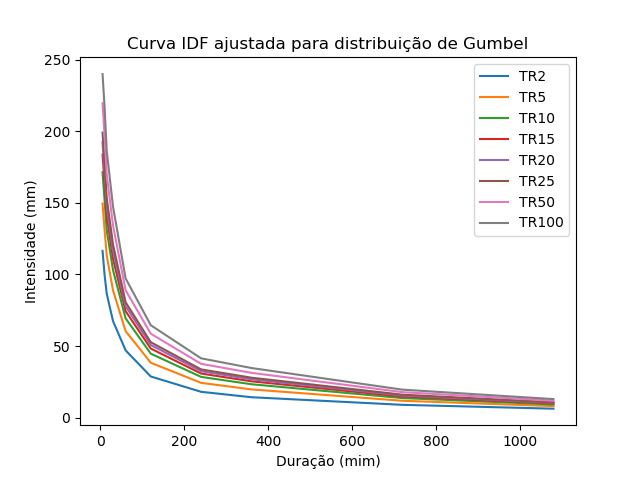
\includegraphics[width=0.8\textwidth]{Textuais/Figuras/curvas-idf-ajustadas.png}
    \fonte{Autores}
    \label{fig:idf-ajustada}
\end{figure}

%rede
\section{Resultados para o modelo de inteligência artificial}

As Figuras \ref{fig:tr2-1n} a \ref{fig:tr100-10n} ilustram as curvas ajustadas para cada período de retorno variando a quantidade de neurônios artificias de 1, 2, 5 e 10 neurônios. Pode-se observar, que a medida em que a quantidade de neurônios é incrementada a saída da rede neural está cada vez mais próxima das intensidades calculadas pela distribuição de Gumbel.

A Tabela \ref{tab:resumo} mostra um resumo dos coeficientes de determinação para cada modelo desse trabalho. Pode-se observar que os valores encontrados pela rede neural estão muito mais próximos da realidade, obtendo uma equação que representa de uma forma mais exata a região de Recife.

\begin{table}[h]
\centering
\caption{Resumo dos coeficientes de determinação para a rede estudada}
\begin{tabular}{@{}ccccccccc@{}}
\toprule
\begin{tabular}[c]{@{}c@{}}Número de \end{tabular} & \multicolumn{8}{c}{Período de Retorno} \\ \cmidrule(l){2-9} 
Neurônios   & 2      & 5      & 10     & 15     & 20     & 25     & 50     & 100    \\ \midrule
1  & 0,9789 & 0,9687 & 0,9654 & 0,9754 & 0,9562 & 0,9658 & 0,9812 & 0,9612 \\
2  & 0,9892 & 0,9756 & 0,9658 & 0,9654 & 0,9654 & 0,9658 & 0,9881 & 0,9781 \\
5  & 0,9951 & 0,9878 & 0,9745 & 0,9851 & 0,9874 & 0,9781 & 0,9956 & 0,9785 \\
10 & 0,9967 & 0,9973 & 0,9856 & 0,9914 & 0,9881 & 0,9789 & 0,9961 & 0,9965 \\ \bottomrule
\end{tabular}
\label{tab:resumo}
\fonte{Autores}
\end{table}

%TR 2
\begin{figure}[h]
    \caption{Curva ajustada para os dados para TR 2 anos e 1 neurônio artificial}
    \centering
    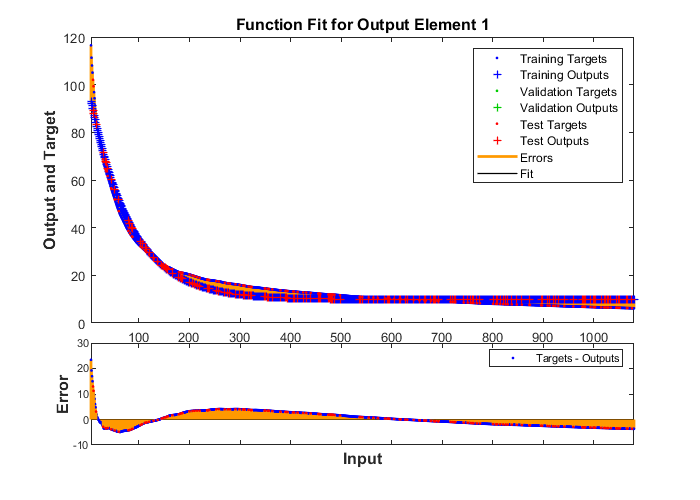
\includegraphics[width=0.74\textwidth]{Textuais/Figuras/NN/tr2-1neuronio.png}
    \fonte{Autores}
    \label{fig:tr2-1n}
\end{figure}

\begin{figure}[h]
    \caption{Curva ajustada para os dados para TR 2 anos e 2 neurônios artificiais}
    \centering
    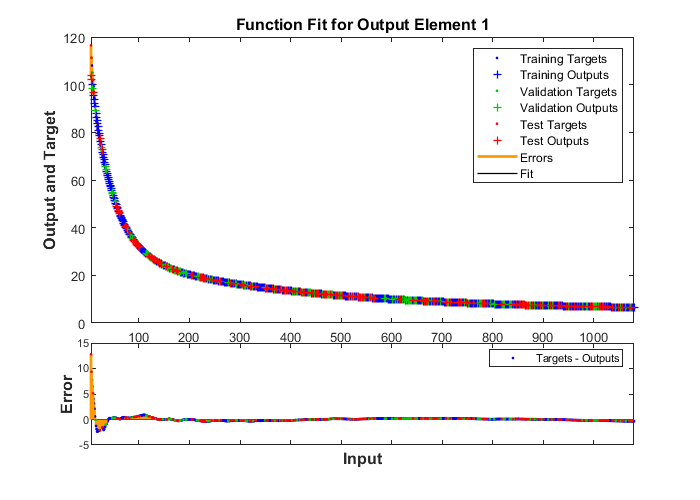
\includegraphics[width=0.74\textwidth]{Textuais/Figuras/NN/tr2-2neuronio.png}
    \fonte{Autores}
    \label{fig:tr2-2n}
\end{figure}

\begin{figure}[h]
    \caption{Curva ajustada para os dados para TR 2 anos e 5 neurônios artificiais}
    \centering
    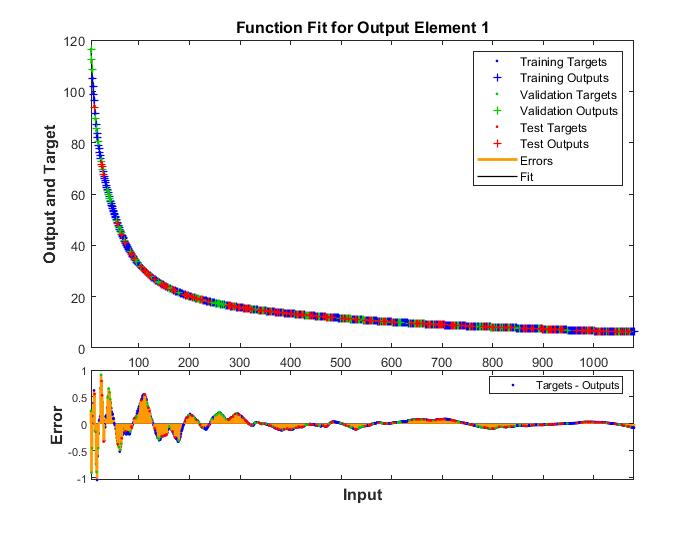
\includegraphics[width=0.74\textwidth]{Textuais/Figuras/NN/tr2-5neuronio.png}
    \fonte{Autores}
    \label{fig:tr2-5n}
\end{figure}

\begin{figure}[h]
    \caption{Curva ajustada para os dados para TR 2 anos e 10 neurônios artificiais}
    \centering
    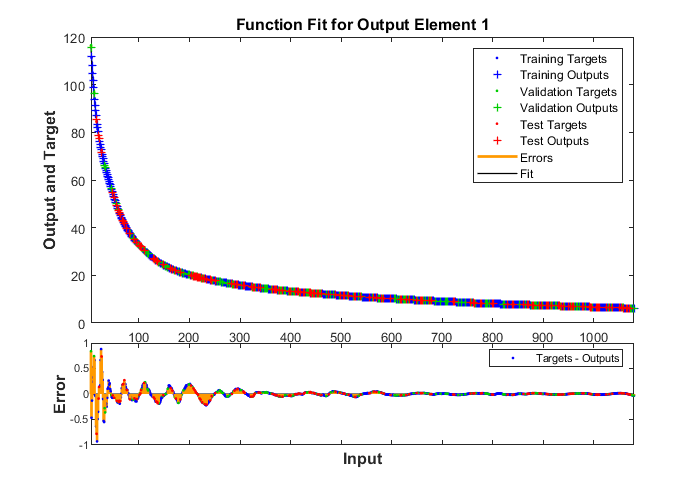
\includegraphics[width=0.74\textwidth]{Textuais/Figuras/NN/tr2-10neuronio.png}
    \fonte{Autores}
    \label{fig:tr2-10n}
\end{figure}
%FIM TR 2

%TR 3
\begin{figure}[h]
    \caption{Curva ajustada para os dados para TR 3 anos e 1 neurônio artificial}
    \centering
    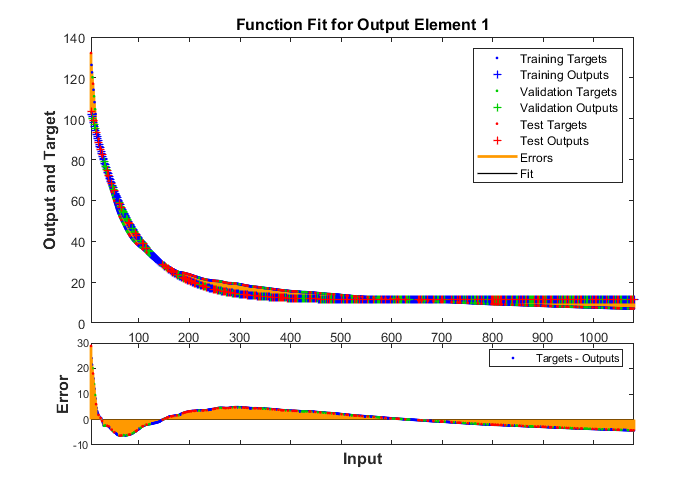
\includegraphics[width=0.74\textwidth]{Textuais/Figuras/NN/tr3-1neuronio.png}
    \fonte{Autores}
    \label{fig:tr3-1n}
\end{figure}

\begin{figure}[h]
    \caption{Curva ajustada para os dados para TR 3 anos e 2 neurônios artificiais}
    \centering
    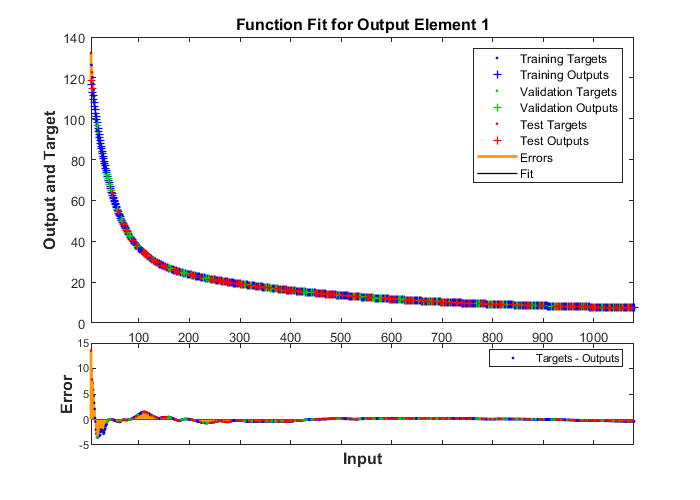
\includegraphics[width=0.74\textwidth]{Textuais/Figuras/NN/tr3-2neuronio.png}
    \fonte{Autores}
    \label{fig:tr3-2n}
\end{figure}

\begin{figure}[h]
    \caption{Curva ajustada para os dados para TR 3 anos e 5 neurônios artificiais}
    \centering
    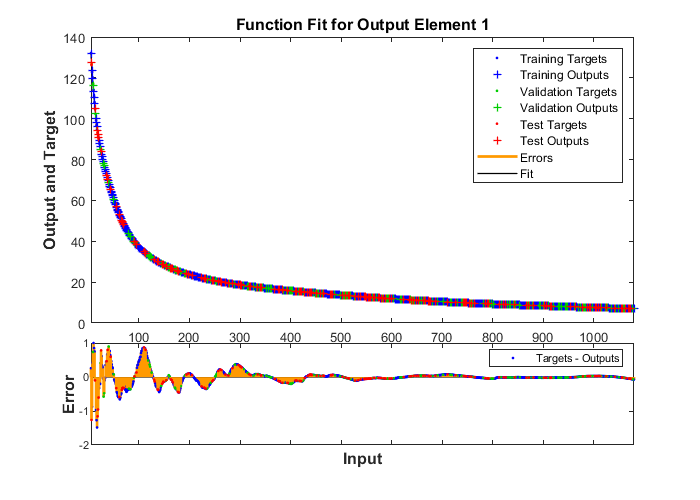
\includegraphics[width=0.74\textwidth]{Textuais/Figuras/NN/tr3-5neuronio.png}
    \fonte{Autores}
    \label{fig:tr3-5n}
\end{figure}

\begin{figure}[h]
    \caption{Curva ajustada para os dados para TR 3 anos e 10 neurônios artificiais}
    \centering
    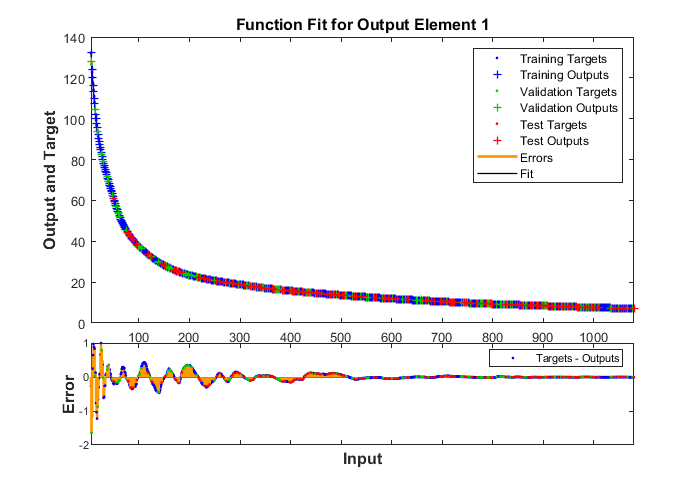
\includegraphics[width=0.74\textwidth]{Textuais/Figuras/NN/tr3-10neuronio.png}
    \fonte{Autores}
    \label{fig:tr3-10n}
\end{figure}
%FIM TR 3

%TR 5
\begin{figure}[h]
    \caption{Curva ajustada para os dados para TR 5 anos e 1 neurônio artificial}
    \centering
    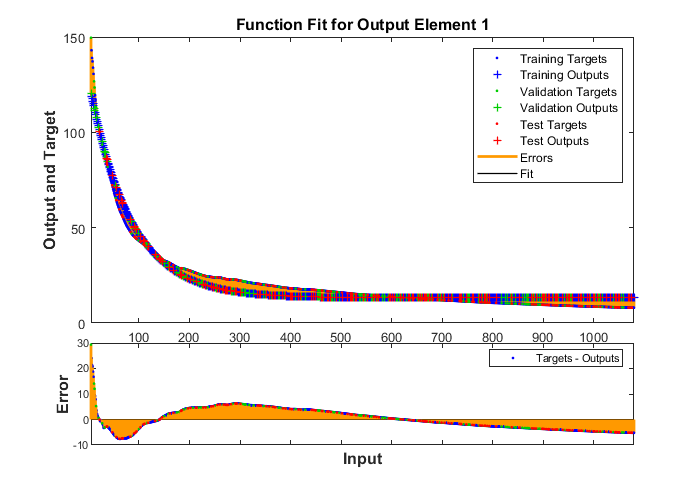
\includegraphics[width=0.74\textwidth]{Textuais/Figuras/NN/tr5-1neuronio.png}
    \fonte{Autores}
    \label{fig:tr5-1n}
\end{figure}

\begin{figure}[h]
    \caption{Curva ajustada para os dados para TR 5 anos e 2 neurônios artificiais}
    \centering
    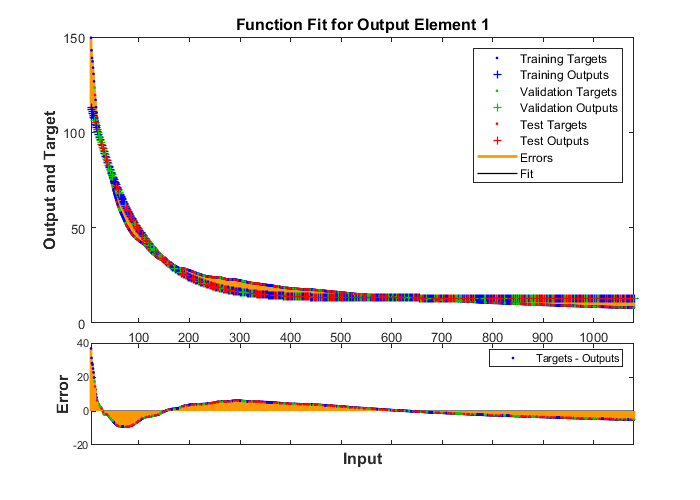
\includegraphics[width=0.74\textwidth]{Textuais/Figuras/NN/tr5-2neuronio.png}
    \fonte{Autores}
    \label{fig:tr5-2n}
\end{figure}

\begin{figure}[h]
    \caption{Curva ajustada para os dados para TR 5 anos e 5 neurônios artificiais}
    \centering
    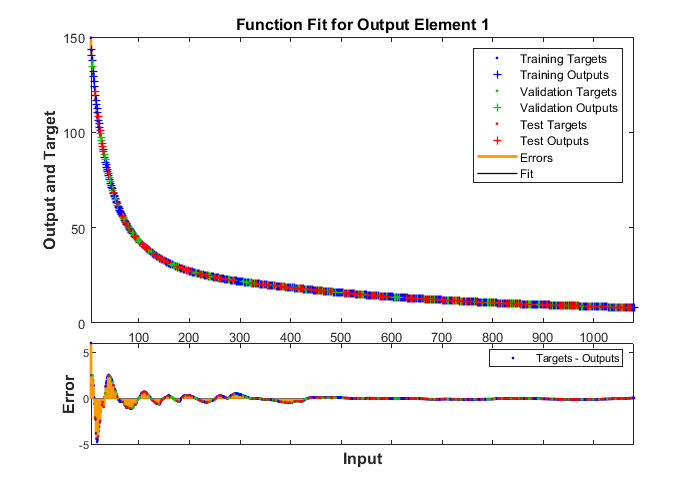
\includegraphics[width=0.74\textwidth]{Textuais/Figuras/NN/tr5-5neuronio.png}
    \fonte{Autores}
    \label{fig:tr5-5n}
\end{figure}

\begin{figure}[h]
    \caption{Curva ajustada para os dados para TR 5 anos e 10 neurônios artificiais}
    \centering
    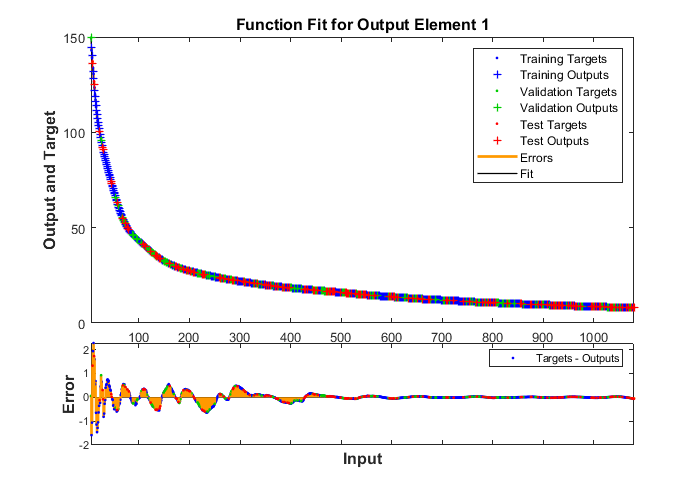
\includegraphics[width=0.74\textwidth]{Textuais/Figuras/NN/tr5-10neuronio.png}
    \fonte{Autores}
    \label{fig:tr5-10n}
\end{figure}
%FIM TR 5

%TR 10
\begin{figure}[h]
    \caption{Curva ajustada para os dados para TR 10 anos e 1 neurônio artificial}
    \centering
    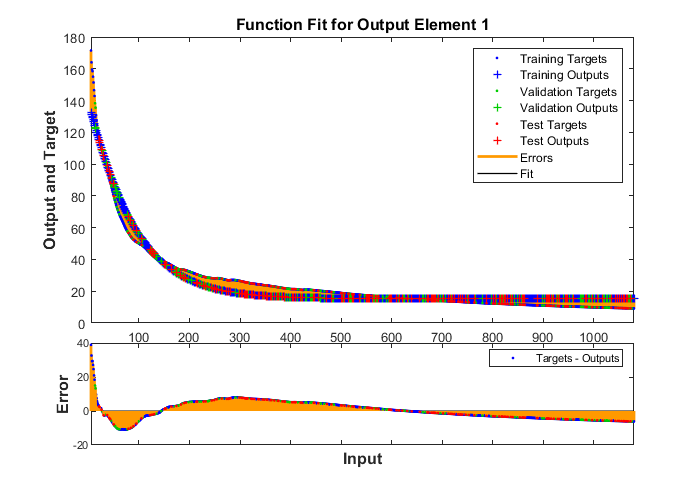
\includegraphics[width=0.74\textwidth]{Textuais/Figuras/NN/tr10-1neuronio.png}
    \fonte{Autores}
    \label{fig:tr10-1n}
\end{figure}

\begin{figure}[h]
    \caption{Curva ajustada para os dados para TR 10 anos e 2 neurônios artificiais}
    \centering
    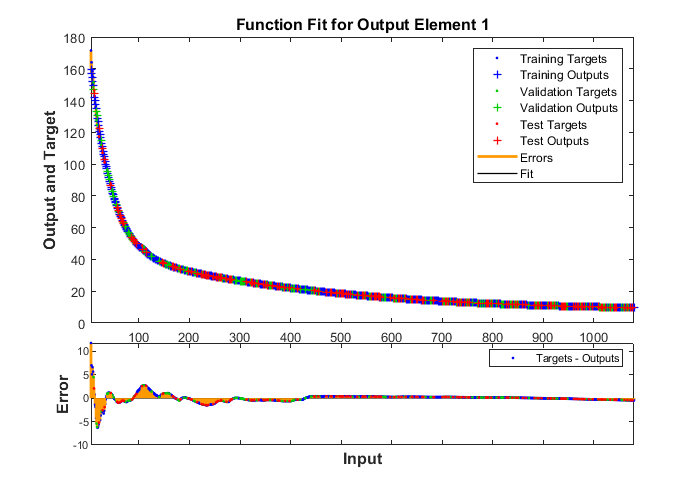
\includegraphics[width=0.74\textwidth]{Textuais/Figuras/NN/tr10-2neuronio.png}
    \fonte{Autores}
    \label{fig:tr10-2n}
\end{figure}

\begin{figure}[h]
    \caption{Curva ajustada para os dados para TR 10 anos e 5 neurônios artificiais}
    \centering
    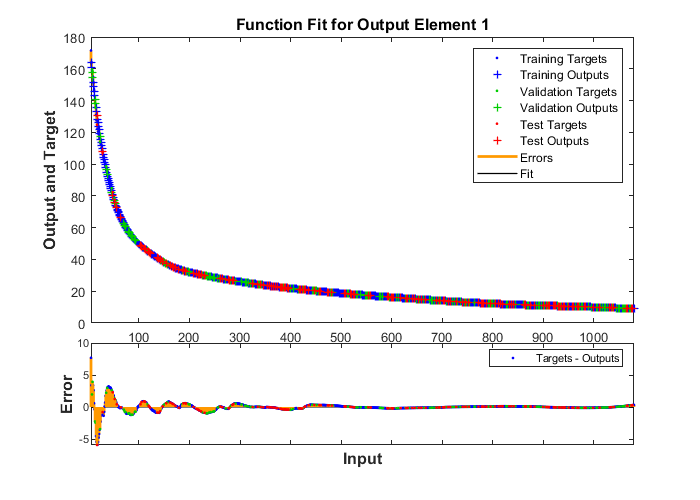
\includegraphics[width=0.74\textwidth]{Textuais/Figuras/NN/tr10-5neuronio.png}
    \fonte{Autores}
    \label{fig:tr10-5n}
\end{figure}

\begin{figure}[h]
    \caption{Curva ajustada para os dados para TR 10 anos e 10 neurônios artificiais}
    \centering
    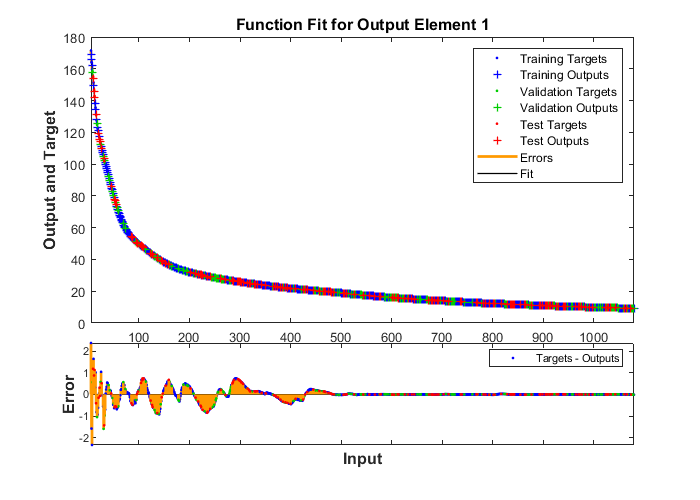
\includegraphics[width=0.74\textwidth]{Textuais/Figuras/NN/tr10-10neuronio.png}
    \fonte{Autores}
    \label{fig:tr10-10n}
\end{figure}
%FIM TR 10

%TR 15
\begin{figure}[h]
    \caption{Curva ajustada para os dados para TR 15 anos e 1 neurônio artificial}
    \centering
    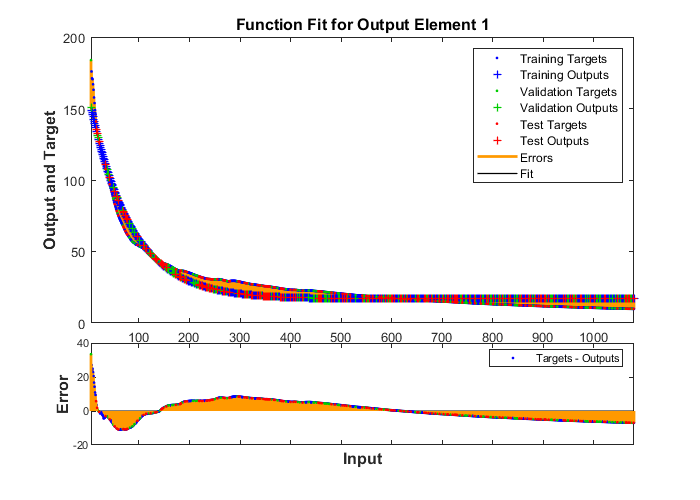
\includegraphics[width=0.74\textwidth]{Textuais/Figuras/NN/tr15-1neuronio.png}
    \fonte{Autores}
    \label{fig:tr15-1n}
\end{figure}

\begin{figure}[h]
    \caption{Curva ajustada para os dados para TR 15 anos e 2 neurônios artificiais}
    \centering
    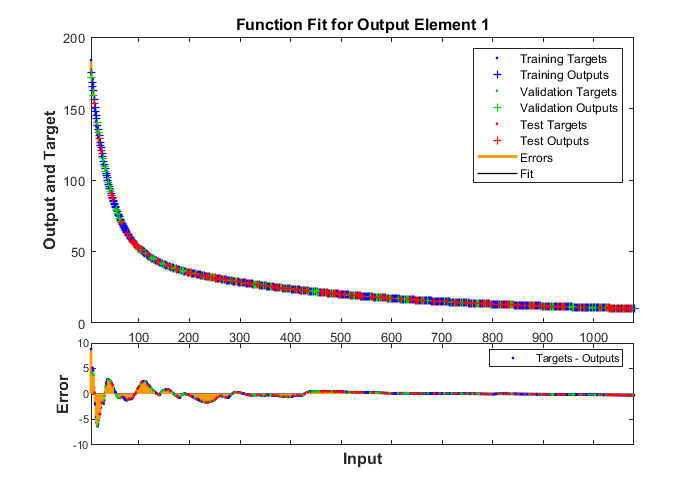
\includegraphics[width=0.74\textwidth]{Textuais/Figuras/NN/tr15-2neuronio.png}
    \fonte{Autores}
    \label{fig:tr15-2n}
\end{figure}

\begin{figure}[h]
    \caption{Curva ajustada para os dados para TR 15 anos e 5 neurônios artificiais}
    \centering
    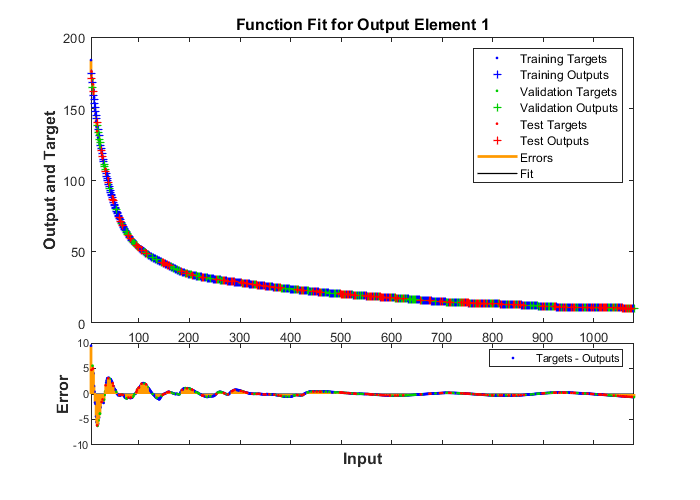
\includegraphics[width=0.74\textwidth]{Textuais/Figuras/NN/tr15-5neuronio.png}
    \fonte{Autores}
    \label{fig:tr15-5n}
\end{figure}

\begin{figure}[h]
    \caption{Curva ajustada para os dados para TR 15 anos e 10 neurônios artificiais}
    \centering
    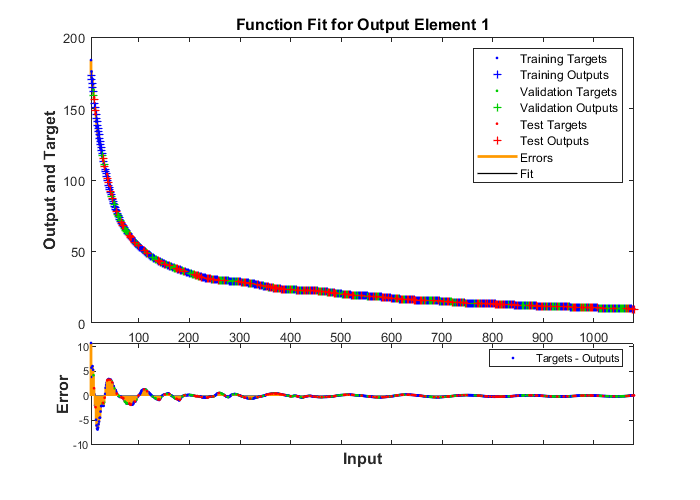
\includegraphics[width=0.74\textwidth]{Textuais/Figuras/NN/tr15-10neuronio.png}
    \fonte{Autores}
    \label{fig:tr15-10n}
\end{figure}
%FIM TR 15

%TR 20
\begin{figure}[h]
    \caption{Curva ajustada para os dados para TR 20 anos e 1 neurônio artificial}
    \centering
    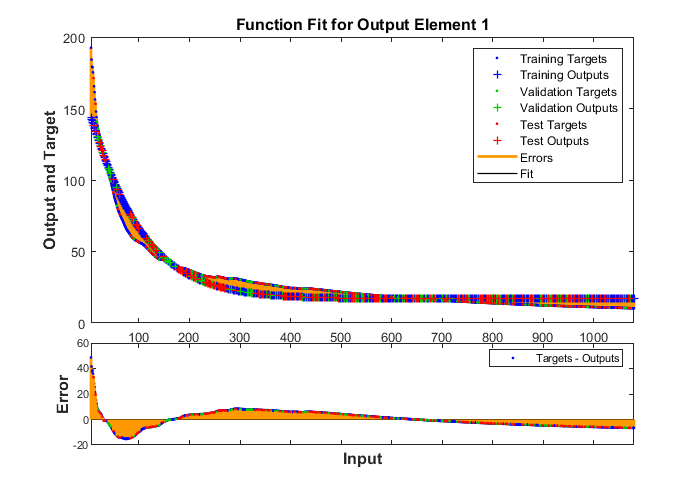
\includegraphics[width=0.74\textwidth]{Textuais/Figuras/NN/tr20-1neuronio.png}
    \fonte{Autores}
    \label{fig:tr20-1n}
\end{figure}

\begin{figure}[h]
    \caption{Curva ajustada para os dados para TR 20 anos e 2 neurônios artificiais}
    \centering
    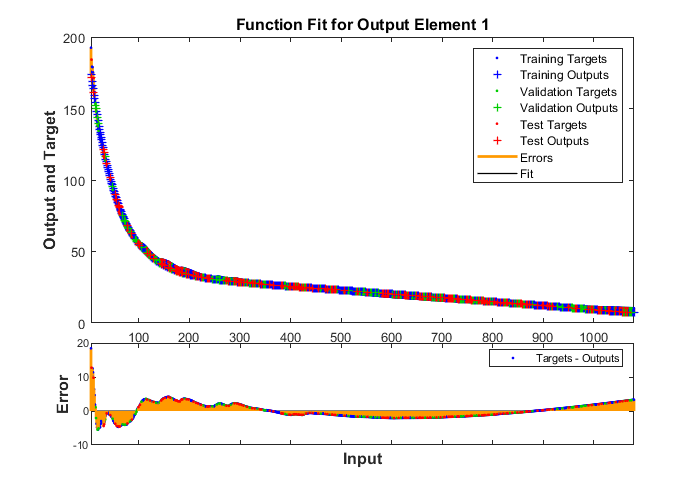
\includegraphics[width=0.74\textwidth]{Textuais/Figuras/NN/tr20-2neuronio.png}
    \fonte{Autores}
    \label{fig:tr20-2n}
\end{figure}

\begin{figure}[h]
    \caption{Curva ajustada para os dados para TR 20 anos e 5 neurônios artificiais}
    \centering
    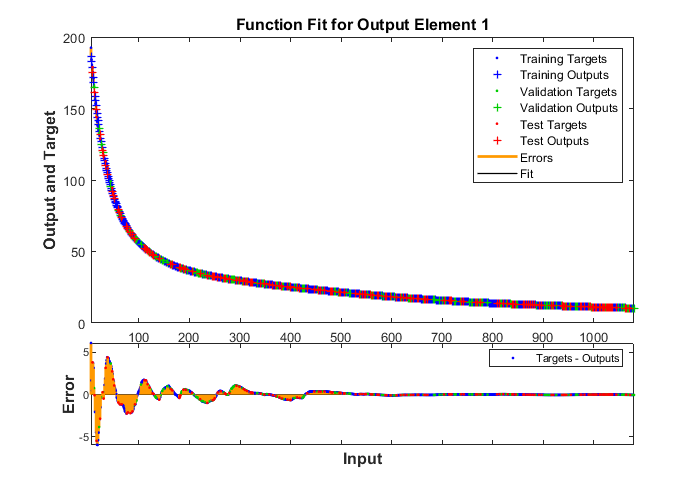
\includegraphics[width=0.74\textwidth]{Textuais/Figuras/NN/tr20-5neuronio.png}
    \fonte{Autores}
    \label{fig:tr20-5n}
\end{figure}

\begin{figure}[h]
    \caption{Curva ajustada para os dados para TR 20 anos e 10 neurônios artificiais}
    \centering
    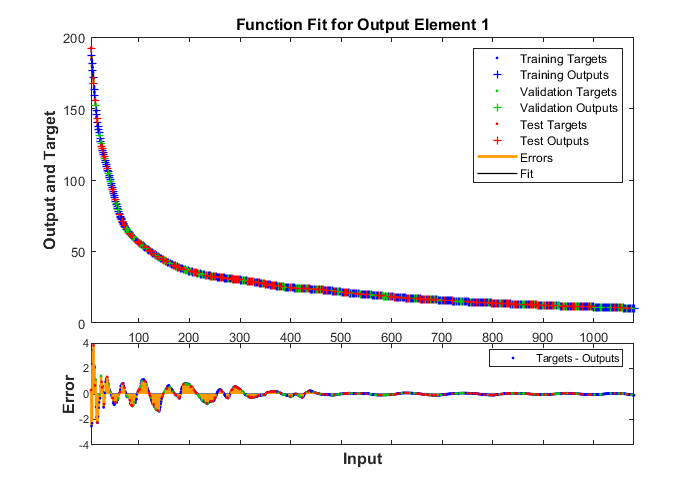
\includegraphics[width=0.74\textwidth]{Textuais/Figuras/NN/tr20-10neuronio.png}
    \fonte{Autores}
    \label{fig:tr20-10n}
\end{figure}
%FIM TR 20

%TR 25
\begin{figure}[h]
    \caption{Curva ajustada para os dados para TR 25 anos e 1 neurônio artificial}
    \centering
    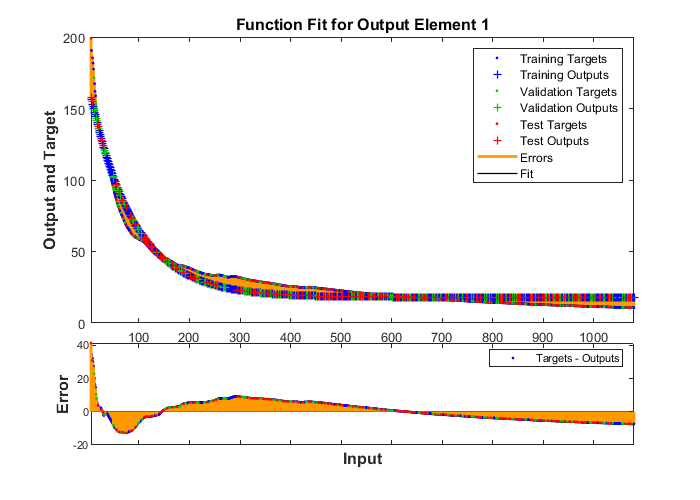
\includegraphics[width=0.74\textwidth]{Textuais/Figuras/NN/tr25-1neuronio.png}
    \fonte{Autores}
    \label{fig:tr25-1n}
\end{figure}

\begin{figure}[h]
    \caption{Curva ajustada para os dados para TR 25 anos e 2 neurônios artificiais}
    \centering
    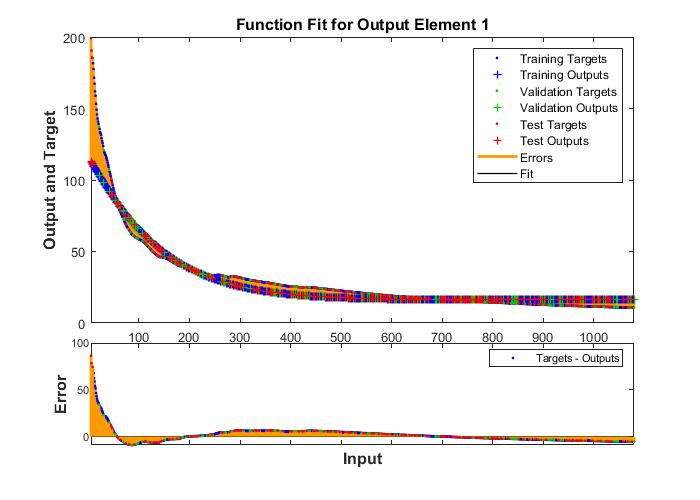
\includegraphics[width=0.74\textwidth]{Textuais/Figuras/NN/tr25-2neuronio.png}
    \fonte{Autores}
    \label{fig:tr25-2n}
\end{figure}

\begin{figure}[h]
    \caption{Curva ajustada para os dados para TR 25 anos e 5 neurônios artificiais}
    \centering
    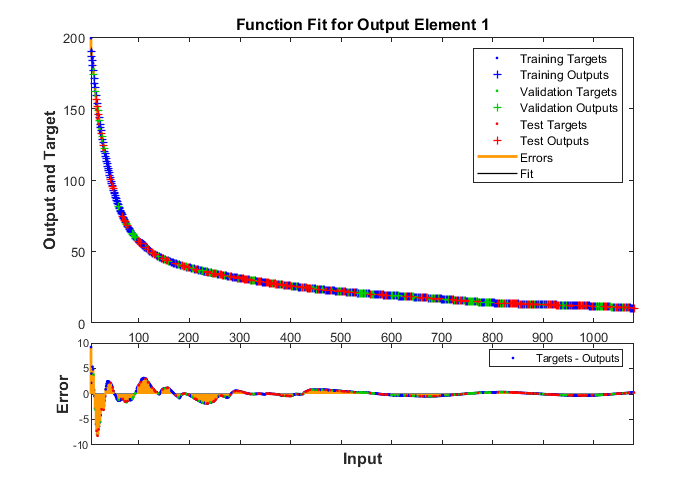
\includegraphics[width=0.74\textwidth]{Textuais/Figuras/NN/tr25-5neuronio.png}
    \fonte{Autores}
    \label{fig:tr25-5n}
\end{figure}

\begin{figure}[h]
    \caption{Curva ajustada para os dados para TR 25 anos e 10 neurônios artificiais}
    \centering
    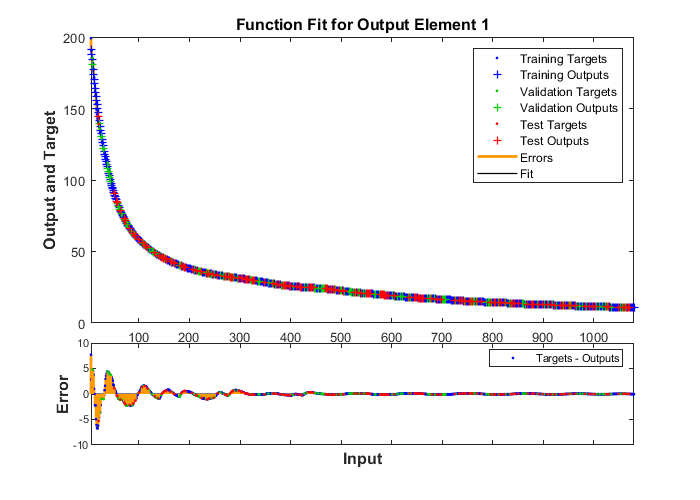
\includegraphics[width=0.74\textwidth]{Textuais/Figuras/NN/tr25-10neuronio.png}
    \fonte{Autores}
    \label{fig:tr25-10n}
\end{figure}
%FIM TR 25

%TR 50
\begin{figure}[h]
    \caption{Curva ajustada para os dados para TR 50 anos e 1 neurônio artificial}
    \centering
    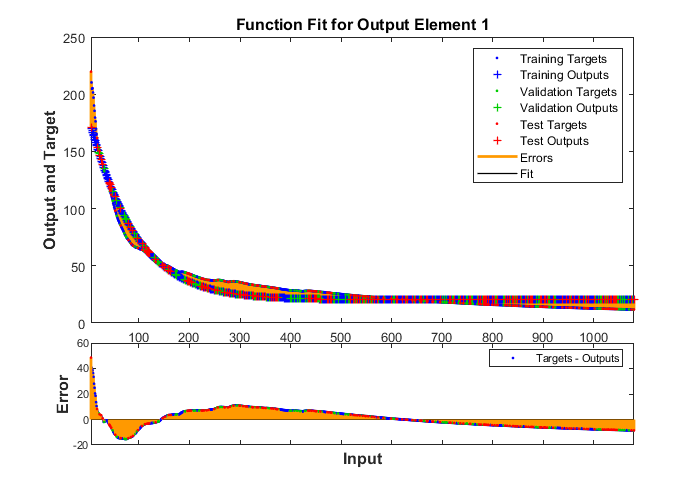
\includegraphics[width=0.74\textwidth]{Textuais/Figuras/NN/tr50-1neuronio.png}
    \fonte{Autores}
    \label{fig:tr50-1n}
\end{figure}

\begin{figure}[h]
    \caption{Curva ajustada para os dados para TR 50 anos e 2 neurônios artificiais}
    \centering
    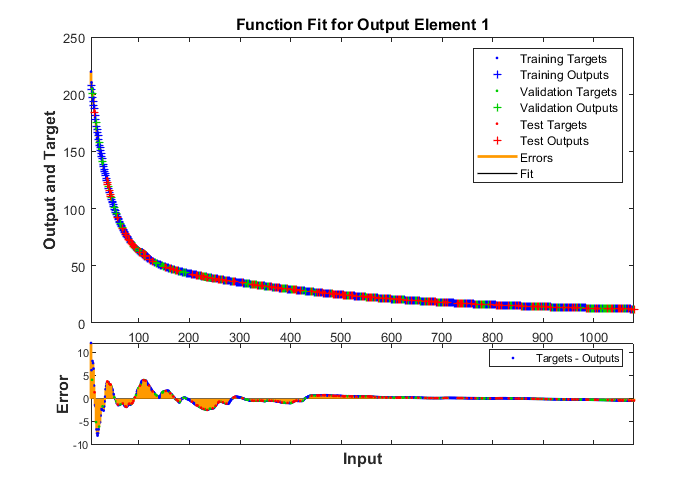
\includegraphics[width=0.74\textwidth]{Textuais/Figuras/NN/tr50-2neuronio.png}
    \fonte{Autores}
    \label{fig:tr50-2n}
\end{figure}

\begin{figure}[h]
    \caption{Curva ajustada para os dados para TR 50 anos e 5 neurônios artificiais}
    \centering
    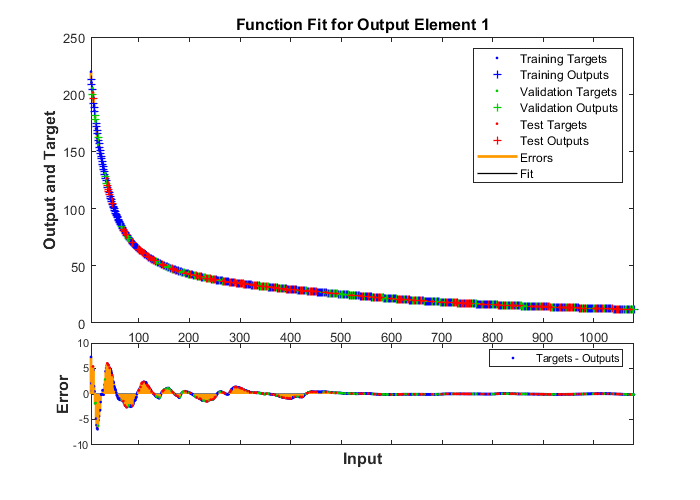
\includegraphics[width=0.74\textwidth]{Textuais/Figuras/NN/tr50-5neuronio.png}
    \fonte{Autores}
    \label{fig:tr50-5n}
\end{figure}

\begin{figure}[h]
    \caption{Curva ajustada para os dados para TR 50 anos e 10 neurônios artificiais}
    \centering
    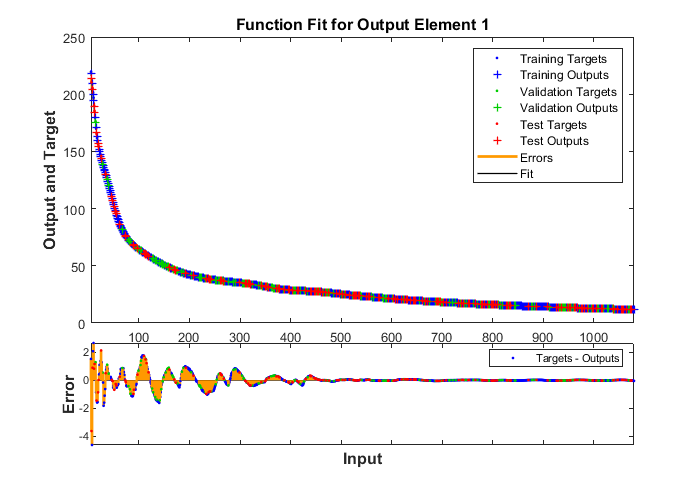
\includegraphics[width=0.74\textwidth]{Textuais/Figuras/NN/tr50-10neuronio.png}
    \fonte{Autores}
    \label{fig:tr50-10n}
\end{figure}
%FIM TR 50

%TR 100
\begin{figure}[h]
    \caption{Curva ajustada para os dados para TR 100 anos e 1 neurônio artificial}
    \centering
    \includegraphics[width=0.74\textwidth]{Textuais/Figuras/NN/tr100-1neuronio.png}
    \fonte{Autores}
    \label{fig:tr100-1n}
\end{figure}

\begin{figure}[h]
    \caption{Curva ajustada para os dados para TR 100 anos e 2 neurônios artificiais}
    \centering
    \includegraphics[width=0.74\textwidth]{Textuais/Figuras/NN/tr100-2neuronio.png}
    \fonte{Autores}
    \label{fig:tr100-2n}
\end{figure}

\begin{figure}[h]
    \caption{Curva ajustada para os dados para TR 100 anos e 5 neurônios artificiais}
    \centering
    \includegraphics[width=0.74\textwidth]{Textuais/Figuras/NN/tr100-5neuronio.png}
    \fonte{Autores}
    \label{fig:tr100-5n}
\end{figure}

\begin{figure}[h]
    \caption{Curva ajustada para os dados para TR 100 anos e 10 neurônios artificiais}
    \centering
    \includegraphics[width=0.74\textwidth]{Textuais/Figuras/NN/tr100-10neuronio.png}
    \fonte{Autores}
    \label{fig:tr100-10n}
\end{figure}
%FIM TR 100


\chapter{Conclusão}

Este trabalho apresentou uma proposta de rede neural artificial recorrente que consegue produzir as curvas de intensidade-duração-frequência para durações entre 5 e 1080 minutos, gerando as curvas para os períodos de retorno de 2, 3, 5, 15, 20, 25, 50 e 100 anos para a cidade de Recife. A série histórica utilizou dados coletados entre os anos 2003 e 2011, pois não apresentavam falhas nas medições. A distribuição de probabilidade de Gumbel mostrou-se representativa para distribuição empírica de probabilidade de eventos extremos para a região escolhida nesse trabalho, comprovada pela aplicação e aprovação no teste estatístico de Kolmogorov-Smirnov a níveis de significância de 1\% e 20\%.

Foi desenvolvido em Matlab a arquitetura da rede neural recorrente utilizando funções de ativação do tipo tangente hiperbólica e algoritmo de Levenberg–Marquardt como método de otimização. Como parâmetro de entrada utilizou-se as durações, e valores de saída as intensidades geradas pela distribuição de probabilidade de Gumbel. Para avaliar a capacidade de aprendizado da rede analisaram-se as saídas para redes compostas por 1, 2, 5 e 10 neurônios de ativação. As seguintes conclusões podem ser destacadas:

\begin{itemize}
    \item A rede neural artificial apresentou coeficientes de determinação entre 0,9789 e 0,9973 para os períodos de retorno entre 2 e 100 anos e durações entre 5 e 1080 minutos, mostrando-se eficiente no caso estudado nesse trabalho.
    \item Os resultados que apresentaram maiores coeficientes de determinação foram para as arquiteturas com 10 neurônios artificiais, atingindo valores de até 0,9973 para o período de retorno de 5 anos.
    \item Até o estudo desse trabalho, a utilização de redes neurais artificiais mostraram-se eficientes para determinação das curvas IDFs.
    \item Pode-se concluir que o número de neurônios impactam no erro final, a medida em que são acrescentados mais neurônios o erro, ao término do aprendizado, é cada vez menor. As RNAs estudadas nesse trabalho, composta por 5 e 10 neurônios, já apresentam desvios inferiores a 0.2\% em comparação as curvas geradas pela Equação de Villela-Mattos (1975). O acréscimo de mais neurônios pode gerar apenas um acréscimo de processamento computacional desnecessário.
\end{itemize}

\section{Trabalhos futuros}

Para dar prosseguimento ao trabalho aqui iniciado, são sugeridos os seguintes estudos futuros:

\begin{enumerate}
    \item Verificar se a rede neural consegue convergir quando as séries históricas contém falhas.
    \item Alterar os parâmetros da rede imputados para verificar a ocorrência de uma possível otimização.
    \item Modificar o algoritmo de convergência para avaliar a forma como a rede irá convergir.
    \item Testar a rede com uma série histórica superior a 30 anos.
    \item Verificar os resultados para diferentes períodos de retorno.
    \item Criar uma nova arquitetura de rede com mais camadas ocultas e outras funções de ativação.
    \item Verificar a capacidade de extrapolação da rede neural artificial.
\end{enumerate}

%Elementos pós-textuais
\postextual
% ----------------------------------------------------------

% ----------------------------------------------------------
% Referências bibliográficas
% ----------------------------------------------------------
\bibliography{Referencias}
%% Glossário
% ----------------------------------------------------------
%
% Consulte o manual da classe abntex2 para orientações sobre o glossário.
%
%\glossary
% Apêndices
% ----------------------------------------------------------

% ---
% Inicia os apêndices
% ---
\begin{apendicesenv}

% Imprime uma página indicando o início dos apêndices
\partapendices

% ----------------------------------------------------------
\chapter{Algoritmo para determinar os parâmetros da equação geral}
% ----------------------------------------------------------

Nesse apêndice é apresentado o código-fonte da implementação computacional em Python para determinar os parâmetros da Equação de Mendes-Ramos.

O código a seguir é responsável pela criação das classes com as máximas intensidades de chuva para cada duração. Também é responsável pela propriedade contendo os períodos de retorno a serem avaliados pela distribuição de Gumbel.

\begin{minted}[mathescape,
               linenos,
               numbersep=5pt,
               gobble=2,
               frame=lines,
               framesep=2mm]{python}
  
    # Data Access Layer
    import numpy as np
    
    class Dados:
        __periodoRetorno = None
        __precipitacao5 = None
        __precipitacao10 = None
        __precipitacao15 = None
        __precipitacao30 = None
        __precipitacao60 = None
        __precipitacao120 = None
        __precipitacao240 = None
        __precipitacao360 = None
        __precipitacao720 = None
        __precipitacao1080 = None
        __duracoes = None
    
        # Construtor - Inicializa os fields da classe
        def __init__(self):
            self.__periodoRetorno = np.array([2, 3, 5, 10, 15, 20, 25, 50, 
            100])
            self.__duracoes = np.array([5, 10, 15, 30, 60, 120, 240, 360, 
            720, 1080])
            self.__precipitacao5 = np.array([7.75, 6.5, 17.25, 8.75, 9.5, 
            11, 9.25, 9.75, 12.25])
            self.__precipitacao10 = np.array([14.25,11.50,29.25,13.25,
            13.00,20.50,15.50,16.50,24.00])
            self.__precipitacao15 = np.array([16.50, 16.50, 36.50, 17.50, 
            17.25, 28.00, 20.25, 20.75, 32.50])
            self.__precipitacao30 = np.array([22.25, 29.50, 51.25, 29.00, 
            26.75, 41.75, 37.75, 26.00, 57.00])
            self.__precipitacao60 = np.array([29.25, 45.25, 69.75, 45.25, 
            40.50, 63.00, 47.50, 33.25, 71.25])
            self.__precipitacao120 = np.array([36.50, 52.25, 102.25, 62.25, 
            41.75, 66.50, 55.50, 44.50, 87.25])
            self.__precipitacao240 = np.array([50.75, 53.50, 137.25, 71.50, 
            47.25, 68.75, 82.00, 77.75, 100.75])
            self.__precipitacao360 = np.array([61.50, 54.00, 176.75, 93.25, 
            56.00, 86.00, 97.25, 95.00, 102.00])
            self.__precipitacao720 = np.array([94.25, 81.00, 206.50, 102.75, 
            73.75, 111.25, 110.50, 112.00, 124.75])
            self.__precipitacao1080 = np.array([100.25, 90.25, 206.50, 102.75, 
            80.75, 112.75, 112.50, 125.00, 125.75])
        
        # Propriedades
        @property
        def get_periodoRetorno(self):
            return self.__periodoRetorno
    
        @property
        def get_precipitacao5(self):
            return self.__precipitacao5
    
        @property
        def get_precipitacao10(self):
            return self.__precipitacao10
    
        @property
        def get_precipitacao15(self):
            return self.__precipitacao15
        
        @property
        def get_precipitacao30(self):
            return self.__precipitacao30
    
        @property
        def get_precipitacao60(self):
            return self.__precipitacao60
    
        @property
        def get_precipitacao120(self):
            return self.__precipitacao120
        
        @property
        def get_precipitacao240(self):
            return self.__precipitacao240
    
        @property
        def get_precipitacao360(self):
            return self.__precipitacao360
    
        @property
        def get_precipitacao720(self):
            return self.__precipitacao720
        
        @property
        def get_precipitacao1080(self):
            return self.__precipitacao1080
    
        @property
        def get_duracoes(self):
            return self.__duracoes
\end{minted}

O código fonte apresentado nas próximas linhas é responsável pela estimativa do coeficiente b da equação idf, fazendo uma iteração entre os valores -100 e 100 até encontrar o melhor valor que torne os dados o mais próximo de uma reta.

\begin{minted}[mathescape,
               linenos,
               numbersep=5pt,
               gobble=2,
               frame=lines,
               framesep=2mm]{python}
    import numpy as np
    from scipy import stats
    
    
    def estimar_b(intensidade, duracao):
        i1 = intensidade[0]
        i2 = intensidade[-1]
        i3 = (i1*i2)**0.5
        t3 = 0
        bi = 0
    
        for i in range(0, len(intensidade)):
            if ((i3<intensidade[i]) and (i3 >= intensidade[i+1])):
                t3 = -((duracao[i]-duracao[i+1])*i3-(duracao[i]*intensidade[i+1]
                -duracao[i+1]*intensidade[i]))/(intensidade[i+1]-intensidade[i])
                bi = ((t3**2)-duracao[0]*duracao[np.size(duracao)-1])/(duracao[0]
                +duracao[np.size(duracao)-1]-2*t3)
                break
        
        b3=[]
    
        for x in range(-100,100):
            if (bi+x >= 0):
                b2 = bi + x
                b3.append(round(b2,0))
            else:
                b2 = 0
                b3.append(b2)
        
        duracao1 = []
        r2_regressao = []
        coef_angular=[]
        coef_linear =[]
    
        for i in range(0,9):
            duracao1.append(duracao + b3[i])
            slope, intercept, r_value, p_value, std_err = 
            regressao_linear(np.log10(duracao1[i]), np.log10(intensidade))
            r2_regressao.append(r_value**2)
            coef_angular.append(slope)
            coef_linear.append(intercept)
        
        r2_max = np.argmax(r2_regressao)
        z = regressao_linear(np.log10(duracao+b3[r2_max]), np.log10(intensidade))
    
        return z, b3[r2_max]
    
    def regressao_linear(x,y):
        return stats.linregress(x, y)
\end{minted}

O próximo código é responsável pela determinação dos outros parâmetros da equação, bem como apresentar o gráfico da curva IDF.

\begin{minted}[mathescape,
               linenos,
               numbersep=5pt,
               gobble=2,
               frame=lines,
               framesep=2mm]{python}
    import dal
    import numpy as np
    import time
    import matplotlib.pyplot as plt
    import precipitacao as prep
    from numpy.linalg import inv
    
    #Inicializa o cronometro para o cálculo do tempo de processamento
    start_time = time.time()
    
    #Instancia a classe com os dados das chuvas
    dados = dal.Dados()
    
    tr = np.array(dados.get_periodoRetorno)
    duracoes = dados.get_duracoes
    
    #Cria uma lista com todas as precipitações
    precipitacoes = np.array([dados.get_precipitacao5, dados.get_precipitacao10, 
    dados.get_precipitacao15, dados.get_precipitacao30, dados.get_precipitacao60, 
    dados.get_precipitacao120, dados.get_precipitacao240, 
    dados.get_precipitacao360, dados.get_precipitacao720, 
    dados.get_precipitacao1080])
    
    precipitacao_decrescente = []
    anos_observados = []
    media_i = []
    desvio_padrao_i = []
    alpha_i = []
    mi_i = []
    gumbel_i = []
    empirica_i = []
    diferenca_gumbel_empirica_i = []
    maxima_diferenca = []
    r2_i = []
    reduzida_gumbel = []
    intensidades = []
    
    for i in range(0, np.size(duracoes)):
        p = prep.Precipitacao(*precipitacoes[i])
        precipitacao_decrescente.append(np.array(p.PrecipitacaoDecrescente()))
        anos_observados.append(p.Anos_Observados) #cte
        media_i.append(p.MediaDuracoes())
        desvio_padrao_i.append(p.DesvioPadrao())
        alpha_i.append(p.ParametroAlpha())
        mi_i.append(p.ParametroMi())
        gumbel_i.append(p.Gumbel())
        empirica_i.append(p.AcumuladaEmpirica()) 
        diferenca_gumbel_empirica_i.append(p.DiferencaTeoricoEmpirico())
        maxima_diferenca.append(p.MaximaDiferenca())
        distribuicoes = {"gumbel" : gumbel_i[i], "empirica" : empirica_i[i]}
        r2_i.append(p.R2(**distribuicoes))
        reduzida_gumbel.append(p.VariavelReduzidaGumbel(tr))
        intensidades.append(p.PrecipitacaoParaIntensidade(duracoes[i], 
        *reduzida_gumbel))
    
    matriz2 = []
    matriz3 = []
    matriz5 = []
    matriz10 = []
    matriz15 = []
    matriz20 = []
    matriz25 = []
    matriz50 = []
    matriz100 = []
    
    for x in range(0, len(duracoes)):
        matriz2.append(intensidades[x][0])
        matriz3.append(intensidades[x][1])
        matriz5.append(intensidades[x][2])
        matriz10.append(intensidades[x][3])
        matriz15.append(intensidades[x][4])
        matriz20.append(intensidades[x][5])
        matriz25.append(intensidades[x][6])
        matriz50.append(intensidades[x][7])
        matriz100.append(intensidades[x][8])
        
    
    plt.figure(1)
    plt.plot(duracoes, matriz2, label="TR2") 
    plt.plot(duracoes, matriz5, label="TR5") 
    plt.plot(duracoes, matriz10, label="TR10") 
    plt.plot(duracoes, matriz15, label="TR15")
    plt.plot(duracoes, matriz20, label="TR20") 
    plt.plot(duracoes, matriz25, label="TR25")
    plt.plot(duracoes, matriz50, label="TR50")
    plt.plot(duracoes, matriz100, label="TR100")
    plt.xlabel("Duração (mim)")
    plt.ylabel("Intensidade (mm)")
    plt.title("Curva IDF ajustada para distribuição de Gumbel")
    plt.legend()
    plt.show()
    
    """plt.figure(2)
    plt.scatter(np.log10(duracoes), np.log10(matriz100), label="TR100")
    plt.xlabel("Duração (mim)")
    plt.ylabel("Intensidade (mm)")
    plt.title("Curva IDF ajustada para distribuição de Gumbel")
    plt.legend()
    plt.show()"""
    
    import estimarb as b
    
    
    b_estimado =[]
    r_quadrado = []
    coef_linear = []
    coef_angular = []
    
    calcular_b = b.estimar_b(matriz2, duracoes)
    coef_angular.append(calcular_b[0][0])
    coef_linear.append(calcular_b[0][1])
    r_quadrado.append(calcular_b[0][2]**2)
    b_estimado.append(calcular_b[1])
    
    calcular_b = b.estimar_b(matriz3, duracoes)
    coef_angular.append(calcular_b[0][0])
    coef_linear.append(calcular_b[0][1])
    r_quadrado.append(calcular_b[0][2]**2)
    b_estimado.append(calcular_b[1])
    
    calcular_b = b.estimar_b(matriz5, duracoes)
    coef_angular.append(calcular_b[0][0])
    coef_linear.append(calcular_b[0][1])
    r_quadrado.append(calcular_b[0][2]**2)
    b_estimado.append(calcular_b[1])
    
    calcular_b = b.estimar_b(matriz10, duracoes)
    coef_angular.append(calcular_b[0][0])
    coef_linear.append(calcular_b[0][1])
    r_quadrado.append(calcular_b[0][2]**2)
    b_estimado.append(calcular_b[1])
    
    calcular_b = b.estimar_b(matriz15, duracoes)
    coef_angular.append(calcular_b[0][0])
    coef_linear.append(calcular_b[0][1])
    r_quadrado.append(calcular_b[0][2]**2)
    b_estimado.append(calcular_b[1])
    
    calcular_b = b.estimar_b(matriz20, duracoes)
    coef_angular.append(calcular_b[0][0])
    coef_linear.append(calcular_b[0][1])
    r_quadrado.append(calcular_b[0][2]**2)
    b_estimado.append(calcular_b[1])
    
    calcular_b = b.estimar_b(matriz25, duracoes)
    coef_angular.append(calcular_b[0][0])
    coef_linear.append(calcular_b[0][1])
    r_quadrado.append(calcular_b[0][2]**2)
    b_estimado.append(calcular_b[1])
    
    calcular_b = b.estimar_b(matriz50, duracoes)
    coef_angular.append(calcular_b[0][0])
    coef_linear.append(calcular_b[0][1])
    r_quadrado.append(calcular_b[0][2]**2)
    b_estimado.append(calcular_b[1])
    
    calcular_b = b.estimar_b(matriz100, duracoes)
    coef_angular.append(calcular_b[0][0])
    coef_linear.append(calcular_b[0][1])
    r_quadrado.append(calcular_b[0][2]**2)
    b_estimado.append(calcular_b[1])
    
    #Regressão múltipla para determinação dos coeficientes
    T = np.size(intensidades)
    b1 = int(0.4 * np.amin(b_estimado))
    b3 = int(1.2 * np.amax(b_estimado))
    b2 = []
    A = np.zeros(shape=(3,3))
    B=[]
    C1=[]
    M1=[]
    N1=[]
    K=[]
    M=[]
    N=[]
    R2 = []
    
    for x in range(b1, b3+1):
        b2.append(x)
    
    numero_de_b = np.size(b2)
    dimensao_gumbel = np.size(intensidades)
    
    for f in range(0, numero_de_b):
        pontos_z_lin = np.asarray(np.log10(intensidades)).reshape(-1) 
        pontos_x_lin = np.repeat(np.log10(duracoes+b2[f]), np.size(tr))
        pontos_y_lin = np.tile(np.log10(tr), np.size(duracoes)) 
    
        A[0,0] = T
        A[0,1] = np.sum(pontos_y_lin)
        A[0,2] = np.sum(pontos_x_lin)
        A[1,0] = np.sum(pontos_y_lin)
        A[1,1] = np.sum(pontos_y_lin * pontos_y_lin)
        A[1,2] = np.sum(pontos_x_lin * pontos_y_lin)
        A[2,0] = np.sum(pontos_x_lin)
        A[2,1] = np.sum(pontos_x_lin * pontos_y_lin)
        A[2,2] = np.sum(pontos_x_lin * pontos_x_lin)
    
        B.clear()
        B.append(np.sum(pontos_z_lin))
        B.append(np.sum(pontos_y_lin * pontos_z_lin))
        B.append(np.sum(pontos_x_lin * pontos_z_lin))
    
        A_inv = inv(A)
    
        solucao = np.linalg.solve(A, B)
    
        C1.append(solucao[0])
        M1.append(solucao[1])
        N1.append(solucao[2])
        K.append(10**C1[f])
        M.append(M1[f])
        N.append(N1[f])
    
        pty=np.tile(tr, np.size(duracoes))
        ptx = np.repeat(duracoes, np.size(tr))
    
        I_est_idf = ((pty ** M[f])*K[f]) * ((ptx+b2[f])**N[f])
    
        an=np.asarray(intensidades).reshape(-1)-
        np.mean(np.asarray(intensidades).reshape(-1))
        bn=I_est_idf-np.mean(I_est_idf)
        R2.append(((np.sum(an*bn)/(np.sum(an**2)*np.sum(bn**2))**0.5))**2)
    
    
    print("Coef K: ", K[np.argmax(R2)])
    print("Coef M: ", M[np.argmax(R2)])
    print("Coef N: ", N[np.argmax(R2)])
    print("Coef b:", b2[np.argmax(R2)])
    print("R2: ", R2[np.argmax(R2)])
    print("--- Tempo de processamento %s segundos ---" % (time.time() - 
    start_time))
\end{minted}

\chapter{Algoritmo para aproximar a função por meio de IA}

Esse apêndice apresenta o algoritmo desenvolvido em Matlab da rede neural recorrente em que as constantes são as que obtiveram o melhor valor do coeficiente de determinação para cada período de retorno. 

\begin{minted}[mathescape,
               linenos,
               numbersep=5pt,
               gobble=2,
               frame=lines,
               framesep=2mm]{matlab}

        function [Y,Xf,Af] = myNeuralNetworkFunction(X,~,~)

        % ===== NEURAL NETWORK CONSTANTS =====
        
        % Input 1
        x1_step1.xoffset = 5;
        x1_step1.gain = 0.00186046511627907;
        x1_step1.ymin = -1;
        
        % Layer 1
        b1 = [11.54090071220356073;8.4772450148319844487;6.5261388646264366642;
        2.9674351566870731389; 1.2178220153517067548;0.70486678409796743594;
        -2.9937829750619364688;-11.148753806533420629;-15.293586250243739855;
        28.530462711213733229];
        IW1_1 = [-12.273804592870089181;-10.800994703366928462;
        -10.180488407919053628;-7.7359047362149384597;-8.2381441164788284937;
        10.987952091508864427;-1.3999111346683161816;-14.016595370202120208;
        -16.56645937666741375;27.549902920393265049];
        
        % Layer 2
        b2 = 8.9148386366500407263;
        LW2_1 = [0.0039532554427080856055 0.0043626122563336922067 
        0.0045844779975845392772 0.009349172795378619949
        0.0054011999595848523073 -0.0049487394160704642823 6.4383624238245396043 
        0.061712764074571817285 0.286809773387178224 -3.0986459999752899996];
        
        % Output 1
        y1_step1.ymin = -1;
        y1_step1.gain = 0.0181283872157426;
        y1_step1.xoffset = 6.187705798;
        
        % ===== SIMULATION ========
        
        % Format Input Arguments
        isCellX = iscell(X);
        if ~isCellX
            X = {X};
        end
        
        % Dimensions
        TS = size(X,2); % timesteps
        if ~isempty(X)
            Q = size(X{1},2); % samples/series
        else
            Q = 0;
        end
        
        % Allocate Outputs
        Y = cell(1,TS);
        
        % Time loop
        for ts=1:TS
            
            % Input 1
            Xp1 = mapminmax_apply(X{1,ts},x1_step1);
            % Layer 1
            a1 = tansig_apply(repmat(b1,1,Q) + IW1_1*Xp1);
            % Layer 2
            a2 = repmat(b2,1,Q) + LW2_1*a1;
            % Output 1
            Y{1,ts} = mapminmax_reverse(a2,y1_step1);
        end
        
        % Final Delay States
        Xf = cell(1,0);
        Af = cell(2,0);
        
        % Format Output Arguments
        if ~isCellX
            Y = cell2mat(Y);
        end
        end
        
        % ===== MODULE FUNCTIONS ========
        
        % Map Minimum and Maximum Input Processing Function
        function y = mapminmax_apply(x,settings)
        y = bsxfun(@minus,x,settings.xoffset);
        y = bsxfun(@times,y,settings.gain);
        y = bsxfun(@plus,y,settings.ymin);
        end
        
        % Sigmoid Symmetric Transfer Function
        function a = tansig_apply(n,~)
        a = 2 ./ (1 + exp(-2*n)) - 1;
        end
        
        % Map Minimum and Maximum Output Reverse-Processing Function
        function x = mapminmax_reverse(y,settings)
        x = bsxfun(@minus,y,settings.ymin);
        x = bsxfun(@rdivide,x,settings.gain);
        x = bsxfun(@plus,x,settings.xoffset);
        end

\end{minted}
\end{apendicesenv}
%% Anexos
% ----------------------------------------------------------

% ---
% Inicia os anexos
% ---
\begin{anexosenv}

% Imprime uma página indicando o início dos anexos
\partanexos

% ---
\chapter{Morbi ultrices rutrum lorem.}
% ---
dsfsd fsd fsd fsd fsdfs df

% ---
\chapter{Cras non urna sed feugiat cum sociis natoque penatibus et magnis dis
parturient montes nascetur ridiculus mus}
% ---

dsfsdf  sdfsdf sdf sdfsd f

% ---
\chapter{Fusce facilisis lacinia dui}
% ---

fsdf sd fsd fsdf sd

\end{anexosenv}
%% ÍNDICE REMISSIVO
%---------------------------------------------------------------------
\phantompart
\printindex

\end{document}
